% lecture5_ro.tex -- GENERATED by build_L5.py from L5_numbers.json; do not edit by hand.
\documentclass[10pt,aspectratio=169,t]{beamer}
% =============================================================================
% emqa_preamble.tex -- shared Beamer preamble of Energy Markets Quantitative Analysis (EMQA)
% Used by every lecture: lectures/Lk/lecturek.tex does
%   \documentclass[10pt,aspectratio=169,t]{beamer}
%   % =============================================================================
% emqa_preamble.tex -- shared Beamer preamble of Energy Markets Quantitative Analysis (EMQA)
% Used by every lecture: lectures/Lk/lecturek.tex does
%   \documentclass[10pt,aspectratio=169,t]{beamer}
%   % =============================================================================
% emqa_preamble.tex -- shared Beamer preamble of Energy Markets Quantitative Analysis (EMQA)
% Used by every lecture: lectures/Lk/lecturek.tex does
%   \documentclass[10pt,aspectratio=169,t]{beamer}
%   \input{../common/emqa_preamble}
%   \emqalecture{k}{Lecture title}
% Logos live in lectures/common/logos/, charts in lectures/Lk/charts/.
% Do NOT add \hfuzz / \vfuzz / \hbadness here: overfull boxes must be fixed, not hidden.
% =============================================================================

\usetheme{default}
\setbeamersize{text margin left=7mm, text margin right=7mm}

% ---------------------------------------------------------------- packages
\usepackage[utf8]{inputenc}
\usepackage[T1]{fontenc}
\usepackage{lmodern}
\usepackage{amsmath, amssymb}
\usepackage{mathtools}
\usepackage{bm}
\usepackage{tikz}
\usetikzlibrary{arrows.meta, positioning, calc, shapes.misc}
\usepackage{booktabs}
\usepackage{array}
\usepackage{graphicx}
\usepackage{colortbl}
\usepackage{xcolor}
\usepackage{multicol}
\hypersetup{colorlinks=true, linkcolor=MainBlue, urlcolor=MainBlue, citecolor=MainBlue}
\graphicspath{{../common/logos/}}   % charts are included with their language folder: charts/en/, charts/ro/

% ---------------------------------------------------------------- colours
\definecolor{MainBlue}{RGB}{26, 58, 110}
\definecolor{IDAred}{RGB}{205, 0, 0}
\definecolor{DarkGray}{RGB}{51, 51, 51}
\definecolor{FooterGray}{RGB}{100, 100, 100}
\definecolor{BlockGray}{RGB}{236, 238, 242}
\definecolor{KeynoteGray}{RGB}{218, 218, 218}
\definecolor{Crimson}{RGB}{190, 40, 50}
\definecolor{Forest}{RGB}{30, 110, 50}
\definecolor{Bitter}{RGB}{214, 150, 20}
% chart palette (same hex values as lectures/common/emqa_plot.py)
\definecolor{SerRO}{HTML}{2A78D6}
\definecolor{SerDE}{HTML}{EB6834}
\definecolor{SerHU}{HTML}{1BAF7A}
\definecolor{SerBG}{HTML}{EDA100}

\setbeamertemplate{background}{%
  \begin{tikzpicture}[remember picture, overlay]
    \shade[shading=axis, shading angle=315, top color=white, bottom color=KeynoteGray]
      (current page.south west) rectangle (current page.north east);
  \end{tikzpicture}}
\setbeamercolor{background canvas}{bg=}
\setbeamercolor{structure}{fg=MainBlue}
\setbeamercolor{normal text}{fg=DarkGray}
\setbeamercolor{title}{fg=IDAred}
\setbeamercolor{frametitle}{fg=IDAred, bg=}
\setbeamercolor{block title}{bg=MainBlue, fg=white}
\setbeamercolor{block body}{bg=BlockGray, fg=DarkGray}
\setbeamercolor{block title alerted}{bg=Crimson, fg=white}
\setbeamercolor{block body alerted}{bg=Crimson!7, fg=DarkGray}
\setbeamercolor{block title example}{bg=Forest, fg=white}
\setbeamercolor{block body example}{bg=Forest!7, fg=DarkGray}
\setbeamercolor{item}{fg=MainBlue}
\setbeamerfont{frametitle}{size=\large, series=\bfseries}
\setbeamerfont{block title}{size=\small, series=\bfseries}
\setbeamertemplate{blocks}[rounded][shadow=false]
\setbeamertemplate{itemize item}{\color{MainBlue}$\boxdot$}
\setbeamertemplate{itemize subitem}{\color{MainBlue}\scriptsize$\blacktriangleright$}
% compact two-level lists: level 1 = main point, level 2 = details (no text outside bullets)
\setbeamerfont{itemize/enumerate subbody}{size=\footnotesize}
\setlength{\leftmargini}{1.1em}
\setlength{\leftmarginii}{1.1em}
\setbeamertemplate{itemize/enumerate body begin}{\setlength{\topsep}{0pt}\setlength{\partopsep}{0pt}\setlength{\parskip}{0pt}}
\setbeamertemplate{itemize/enumerate subbody begin}{\setlength{\topsep}{0pt}\setlength{\partopsep}{0pt}\setlength{\itemsep}{0pt}\vspace{-0.4ex}}

\setbeamertemplate{enumerate item}{\color{MainBlue}\insertenumlabel.}
\setlength{\leftmargini}{1.3em}
\setlength{\leftmarginii}{1.2em}
\setbeamertemplate{navigation symbols}{}
\setbeamertemplate{section in toc}{\color{MainBlue}$\blacktriangleright$~\inserttocsection}
\setbeamertemplate{caption}{\raggedright\insertcaption\par}
% frame subtitle = precise citation line under the claim title (Weron style)
\setbeamerfont{framesubtitle}{size=\footnotesize}
\setbeamercolor{framesubtitle}{fg=FooterGray}
% outline that reappears at every section with the current section highlighted
\setbeamertemplate{section in toc shaded}[default][35]
\setbeamertemplate{subsection in toc shaded}[default][35]
\setbeamertemplate{subsection in toc}{\leavevmode\leftskip=2.2em\color{DarkGray}\small\inserttocsubsection\par}
\AtBeginSection[]{{\begin{frame}{\txtoutline}\vspace{2mm}\small
  \tableofcontents[currentsection,hideothersubsections]\end{frame}}}

% ---------------------------------------------------------------- head and foot
\setbeamertemplate{headline}{%
  \vskip10pt%
  \hbox to \paperwidth{\hskip0.5cm%
    {\small\color{FooterGray}\renewcommand{\hyperlink}[2]{##2}\insertsectionhead}%
    \hfill\textcolor{FooterGray}{\small\insertframenumber}\hskip0.5cm}%
  \vskip4pt{\color{FooterGray}\hrule height 0.4pt}}
% footer as in the other courses (MFM, SFM): course name on the left, small sparkline on the right
\setbeamertemplate{footline}{%
  {\color{FooterGray}\hrule height 0.4pt}\vskip4pt%
  \hbox to \paperwidth{\hskip0.5cm%
    \textcolor{FooterGray}{\small\txtcourse}%
    \hfill\raisebox{-0.1em}{\begin{tikzpicture}[x=0.08em, y=0.08em, line width=0.4pt]
      \draw[FooterGray] (0,3) -- (1,4) -- (2,3.5) -- (3,5) -- (4,4) -- (5,6) -- (6,5.5) -- (7,4) -- (8,5) -- (9,7) -- (10,6) -- (11,5) -- (12,6.5) -- (13,8) -- (14,7) -- (15,6) -- (16,7.5) -- (17,9) -- (18,8) -- (19,7) -- (20,8.5) -- (21,10) -- (22,9) -- (23,8) -- (24,9.5);
    \end{tikzpicture}}\hskip0.5cm}%
  \vskip6pt}

% ---------------------------------------------------------------- title page
\defbeamertemplate*{title page}{emqa}[1][]{%
  \vspace{0.15cm}
  \begin{center}
    \href{https://www.ase.ro}{
\includegraphics[height=0.9cm]{ase_logo.png}}\hspace{0.3cm}%
    \href{https://ipe.ro/new}{
\includegraphics[height=0.9cm]{acad_logo.png}}\hspace{0.3cm}%
    \href{https://theida.net}{
\includegraphics[height=0.9cm]{ida_logo.png}}\hspace{0.3cm}%
    \href{https://blockchain-research-center.com}{
\includegraphics[height=0.9cm]{brc_logo.png}}\hspace{0.3cm}%
    \href{https://www.ai4efin.ase.ro}{
\includegraphics[height=0.9cm]{ai4efin_logo.png}}\hspace{0.3cm}%
    \href{https://www.digital-finance-msca.com}{
\includegraphics[height=0.9cm]{msca_logo.png}}%
  \end{center}
  \vspace{0.45cm}
  \begin{center}
    \begin{minipage}{0.1\textwidth}\centering
      \href{https://quantlet.com}{
\includegraphics[height=0.9cm]{ql_logo.png}}\end{minipage}%
    \begin{minipage}{0.78\textwidth}\centering
      {\Large\bfseries\usebeamercolor[fg]{title}\inserttitle}\par\vspace{0.25cm}
      {\large\usebeamercolor[fg]{title}\insertsubtitle}\end{minipage}%
    \begin{minipage}{0.1\textwidth}\centering
      \href{https://quantinar.com}{
\includegraphics[height=0.9cm]{qr_logo.png}}\end{minipage}
  \end{center}
  \vfill
  \hspace{0.4cm}{\bfseries\insertauthor}\par\vspace{0.12cm}
  \hspace{0.4cm}\begin{minipage}[t]{0.92\textwidth}\raggedright\footnotesize\insertinstitute\end{minipage}
  \par\vspace{0.4cm}}

% ---------------------------------------------------------------- lecture metadata
\newcommand{\emqashort}{}
\newcommand{\emqanb}{notebooks}
\newcommand{\emqarepo}{https://github.com/danpele/EMQA/tree/main}
% language-dependent labels (English default; \emqaromanian switches to Romanian, call it before \emqalecture)
\newcommand{\txtcourse}{Energy Markets Quantitative Analysis}
\newcommand{\txtlecture}{Lecture}
\newcommand{\txtoutline}{Outline}
\newcommand{\txtintuition}{In one sentence:}
\newcommand{\txtjob}{In practice:}
\newcommand{\txttry}{Experiment yourself:}
\newcommand{\txtwhere}{where}
\newcommand{\txtsim}{SIMULATED DATA (teaching illustration)}
\newcommand{\txtnbsuffix}{}
\newcommand{\txtinstitute}{Bucharest University of Economic Studies, Department of Statistics and Econometrics\\
    Romanian Academy, Institute for Economic Forecasting\\
    IDA Institute Digital Assets \textbullet\ AI4EFin \textbullet\ MSCA Digital Finance}
\newcommand{\emqaromanian}{%
  \renewcommand{\txtcourse}{Analiza cantitativă a piețelor de energie}%
  \renewcommand{\txtlecture}{Cursul}%
  \renewcommand{\txtoutline}{Cuprins}%
  \renewcommand{\txtintuition}{Pe scurt:}%
  \renewcommand{\txtjob}{În practică:}%
  \renewcommand{\txttry}{Exercițiu practic:}%
  \renewcommand{\txtwhere}{unde}%
  \renewcommand{\txtsim}{DATE SIMULATE (doar pentru ilustrare)}%
  \renewcommand{\txtnbsuffix}{\string_ro}%
  \renewcommand{\txtinstitute}{Academia de Studii Economice din București, Departamentul de Statistică și Econometrie\\
    Academia Română, Institutul de Prognoză Economică\\
    IDA Institute Digital Assets \textbullet\ AI4EFin \textbullet\ MSCA Digital Finance}}
\newcommand{\emqalecture}[2]{%
  \renewcommand{\emqashort}{\txtlecture\ #1}%
  \renewcommand{\emqanb}{notebooks/L#1\string_notebook\txtnbsuffix.ipynb}%
  \title[EMQA]{\txtcourse}%
  \subtitle{\txtlecture\ #1: #2}%
  \author{Prof.\ dr.\ Daniel Traian PELE}%
  \institute{\txtinstitute}%
  \date{}}

% ---------------------------------------------------------------- teaching blocks (MBA clarity rule)
% \intuition{one plain sentence}  ->  formula with every symbol defined  ->  real-data example  ->  \manager{one line}
\newcommand{\intuition}[1]{\begin{itemize}\item {\color{MainBlue}\textbf{\txtintuition}}~#1\end{itemize}\vspace{0.6mm}}
\newcommand{\manager}[1]{\colorbox{Forest!10}{\parbox{\dimexpr\linewidth-2\fboxsep\relax}{\footnotesize
  \begin{itemize}\setlength{\itemsep}{0pt}\item \textbf{\color{Forest}\txtjob}~#1\end{itemize}}}}
% Experiment yourself: pointer to the matching notebook section
\newcommand{\tryit}[1]{{\scriptsize\href{\emqarepo/\emqanb}{%
  \raisebox{-0.15em}{
\includegraphics[height=0.85em]{ql_logo.png}}\,\textbf{\txttry}~\color{MainBlue}#1}}}
% bottom row: manager line (left) + experiment pointer (right), pinned to the bottom of the frame
\newcommand{\bottomrow}[2]{\par\vfill\noindent\begin{minipage}[b]{0.72\linewidth}#1\end{minipage}\hfill
  \begin{minipage}[b]{0.26\linewidth}\raggedleft #2\end{minipage}\par\vspace{0.5mm}}
\newcommand{\where}[1]{{\footnotesize\textbf{\txtwhere}~#1\par}}

% ---------------------------------------------------------------- helpers
% chart source line under a figure: \chartsource{Source ...; period ...}
\newcommand{\chartsource}[1]{\par\vspace{1pt}{\scriptsize\color{FooterGray}#1\par}}
% link to code: \quantlet{label}{path inside the repo}
\newcommand{\quantlet}[2]{\par\vspace{1pt}\hfill\href{\emqarepo/#2}{%
  \raisebox{-0.15em}{
\includegraphics[height=0.75em]{ql_logo.png}}\textcolor{MainBlue}{\scriptsize\ #1}}}
\newcommand{\simlabel}{\colorbox{Crimson!12}{\scriptsize\bfseries\color{Crimson}\txtsim}}
\newcommand{\E}{\mathbb{E}}
\newcommand{\Var}{\operatorname{Var}}
\newcommand{\Cov}{\operatorname{Cov}}
\newcommand{\Corr}{\operatorname{Corr}}
\newcommand{\asinh}{\operatorname{asinh}}
\newcommand{\iid}{\overset{\text{i.i.d.}}{\sim}}
\newcommand{\EUR}{EUR}

%   \emqalecture{k}{Lecture title}
% Logos live in lectures/common/logos/, charts in lectures/Lk/charts/.
% Do NOT add \hfuzz / \vfuzz / \hbadness here: overfull boxes must be fixed, not hidden.
% =============================================================================

\usetheme{default}
\setbeamersize{text margin left=7mm, text margin right=7mm}

% ---------------------------------------------------------------- packages
\usepackage[utf8]{inputenc}
\usepackage[T1]{fontenc}
\usepackage{lmodern}
\usepackage{amsmath, amssymb}
\usepackage{mathtools}
\usepackage{bm}
\usepackage{tikz}
\usetikzlibrary{arrows.meta, positioning, calc, shapes.misc}
\usepackage{booktabs}
\usepackage{array}
\usepackage{graphicx}
\usepackage{colortbl}
\usepackage{xcolor}
\usepackage{multicol}
\hypersetup{colorlinks=true, linkcolor=MainBlue, urlcolor=MainBlue, citecolor=MainBlue}
\graphicspath{{../common/logos/}}   % charts are included with their language folder: charts/en/, charts/ro/

% ---------------------------------------------------------------- colours
\definecolor{MainBlue}{RGB}{26, 58, 110}
\definecolor{IDAred}{RGB}{205, 0, 0}
\definecolor{DarkGray}{RGB}{51, 51, 51}
\definecolor{FooterGray}{RGB}{100, 100, 100}
\definecolor{BlockGray}{RGB}{236, 238, 242}
\definecolor{KeynoteGray}{RGB}{218, 218, 218}
\definecolor{Crimson}{RGB}{190, 40, 50}
\definecolor{Forest}{RGB}{30, 110, 50}
\definecolor{Bitter}{RGB}{214, 150, 20}
% chart palette (same hex values as lectures/common/emqa_plot.py)
\definecolor{SerRO}{HTML}{2A78D6}
\definecolor{SerDE}{HTML}{EB6834}
\definecolor{SerHU}{HTML}{1BAF7A}
\definecolor{SerBG}{HTML}{EDA100}

\setbeamertemplate{background}{%
  \begin{tikzpicture}[remember picture, overlay]
    \shade[shading=axis, shading angle=315, top color=white, bottom color=KeynoteGray]
      (current page.south west) rectangle (current page.north east);
  \end{tikzpicture}}
\setbeamercolor{background canvas}{bg=}
\setbeamercolor{structure}{fg=MainBlue}
\setbeamercolor{normal text}{fg=DarkGray}
\setbeamercolor{title}{fg=IDAred}
\setbeamercolor{frametitle}{fg=IDAred, bg=}
\setbeamercolor{block title}{bg=MainBlue, fg=white}
\setbeamercolor{block body}{bg=BlockGray, fg=DarkGray}
\setbeamercolor{block title alerted}{bg=Crimson, fg=white}
\setbeamercolor{block body alerted}{bg=Crimson!7, fg=DarkGray}
\setbeamercolor{block title example}{bg=Forest, fg=white}
\setbeamercolor{block body example}{bg=Forest!7, fg=DarkGray}
\setbeamercolor{item}{fg=MainBlue}
\setbeamerfont{frametitle}{size=\large, series=\bfseries}
\setbeamerfont{block title}{size=\small, series=\bfseries}
\setbeamertemplate{blocks}[rounded][shadow=false]
\setbeamertemplate{itemize item}{\color{MainBlue}$\boxdot$}
\setbeamertemplate{itemize subitem}{\color{MainBlue}\scriptsize$\blacktriangleright$}
% compact two-level lists: level 1 = main point, level 2 = details (no text outside bullets)
\setbeamerfont{itemize/enumerate subbody}{size=\footnotesize}
\setlength{\leftmargini}{1.1em}
\setlength{\leftmarginii}{1.1em}
\setbeamertemplate{itemize/enumerate body begin}{\setlength{\topsep}{0pt}\setlength{\partopsep}{0pt}\setlength{\parskip}{0pt}}
\setbeamertemplate{itemize/enumerate subbody begin}{\setlength{\topsep}{0pt}\setlength{\partopsep}{0pt}\setlength{\itemsep}{0pt}\vspace{-0.4ex}}

\setbeamertemplate{enumerate item}{\color{MainBlue}\insertenumlabel.}
\setlength{\leftmargini}{1.3em}
\setlength{\leftmarginii}{1.2em}
\setbeamertemplate{navigation symbols}{}
\setbeamertemplate{section in toc}{\color{MainBlue}$\blacktriangleright$~\inserttocsection}
\setbeamertemplate{caption}{\raggedright\insertcaption\par}
% frame subtitle = precise citation line under the claim title (Weron style)
\setbeamerfont{framesubtitle}{size=\footnotesize}
\setbeamercolor{framesubtitle}{fg=FooterGray}
% outline that reappears at every section with the current section highlighted
\setbeamertemplate{section in toc shaded}[default][35]
\setbeamertemplate{subsection in toc shaded}[default][35]
\setbeamertemplate{subsection in toc}{\leavevmode\leftskip=2.2em\color{DarkGray}\small\inserttocsubsection\par}
\AtBeginSection[]{{\begin{frame}{\txtoutline}\vspace{2mm}\small
  \tableofcontents[currentsection,hideothersubsections]\end{frame}}}

% ---------------------------------------------------------------- head and foot
\setbeamertemplate{headline}{%
  \vskip10pt%
  \hbox to \paperwidth{\hskip0.5cm%
    {\small\color{FooterGray}\renewcommand{\hyperlink}[2]{##2}\insertsectionhead}%
    \hfill\textcolor{FooterGray}{\small\insertframenumber}\hskip0.5cm}%
  \vskip4pt{\color{FooterGray}\hrule height 0.4pt}}
% footer as in the other courses (MFM, SFM): course name on the left, small sparkline on the right
\setbeamertemplate{footline}{%
  {\color{FooterGray}\hrule height 0.4pt}\vskip4pt%
  \hbox to \paperwidth{\hskip0.5cm%
    \textcolor{FooterGray}{\small\txtcourse}%
    \hfill\raisebox{-0.1em}{\begin{tikzpicture}[x=0.08em, y=0.08em, line width=0.4pt]
      \draw[FooterGray] (0,3) -- (1,4) -- (2,3.5) -- (3,5) -- (4,4) -- (5,6) -- (6,5.5) -- (7,4) -- (8,5) -- (9,7) -- (10,6) -- (11,5) -- (12,6.5) -- (13,8) -- (14,7) -- (15,6) -- (16,7.5) -- (17,9) -- (18,8) -- (19,7) -- (20,8.5) -- (21,10) -- (22,9) -- (23,8) -- (24,9.5);
    \end{tikzpicture}}\hskip0.5cm}%
  \vskip6pt}

% ---------------------------------------------------------------- title page
\defbeamertemplate*{title page}{emqa}[1][]{%
  \vspace{0.15cm}
  \begin{center}
    \href{https://www.ase.ro}{
\includegraphics[height=0.9cm]{ase_logo.png}}\hspace{0.3cm}%
    \href{https://ipe.ro/new}{
\includegraphics[height=0.9cm]{acad_logo.png}}\hspace{0.3cm}%
    \href{https://theida.net}{
\includegraphics[height=0.9cm]{ida_logo.png}}\hspace{0.3cm}%
    \href{https://blockchain-research-center.com}{
\includegraphics[height=0.9cm]{brc_logo.png}}\hspace{0.3cm}%
    \href{https://www.ai4efin.ase.ro}{
\includegraphics[height=0.9cm]{ai4efin_logo.png}}\hspace{0.3cm}%
    \href{https://www.digital-finance-msca.com}{
\includegraphics[height=0.9cm]{msca_logo.png}}%
  \end{center}
  \vspace{0.45cm}
  \begin{center}
    \begin{minipage}{0.1\textwidth}\centering
      \href{https://quantlet.com}{
\includegraphics[height=0.9cm]{ql_logo.png}}\end{minipage}%
    \begin{minipage}{0.78\textwidth}\centering
      {\Large\bfseries\usebeamercolor[fg]{title}\inserttitle}\par\vspace{0.25cm}
      {\large\usebeamercolor[fg]{title}\insertsubtitle}\end{minipage}%
    \begin{minipage}{0.1\textwidth}\centering
      \href{https://quantinar.com}{
\includegraphics[height=0.9cm]{qr_logo.png}}\end{minipage}
  \end{center}
  \vfill
  \hspace{0.4cm}{\bfseries\insertauthor}\par\vspace{0.12cm}
  \hspace{0.4cm}\begin{minipage}[t]{0.92\textwidth}\raggedright\footnotesize\insertinstitute\end{minipage}
  \par\vspace{0.4cm}}

% ---------------------------------------------------------------- lecture metadata
\newcommand{\emqashort}{}
\newcommand{\emqanb}{notebooks}
\newcommand{\emqarepo}{https://github.com/danpele/EMQA/tree/main}
% language-dependent labels (English default; \emqaromanian switches to Romanian, call it before \emqalecture)
\newcommand{\txtcourse}{Energy Markets Quantitative Analysis}
\newcommand{\txtlecture}{Lecture}
\newcommand{\txtoutline}{Outline}
\newcommand{\txtintuition}{In one sentence:}
\newcommand{\txtjob}{In practice:}
\newcommand{\txttry}{Experiment yourself:}
\newcommand{\txtwhere}{where}
\newcommand{\txtsim}{SIMULATED DATA (teaching illustration)}
\newcommand{\txtnbsuffix}{}
\newcommand{\txtinstitute}{Bucharest University of Economic Studies, Department of Statistics and Econometrics\\
    Romanian Academy, Institute for Economic Forecasting\\
    IDA Institute Digital Assets \textbullet\ AI4EFin \textbullet\ MSCA Digital Finance}
\newcommand{\emqaromanian}{%
  \renewcommand{\txtcourse}{Analiza cantitativă a piețelor de energie}%
  \renewcommand{\txtlecture}{Cursul}%
  \renewcommand{\txtoutline}{Cuprins}%
  \renewcommand{\txtintuition}{Pe scurt:}%
  \renewcommand{\txtjob}{În practică:}%
  \renewcommand{\txttry}{Exercițiu practic:}%
  \renewcommand{\txtwhere}{unde}%
  \renewcommand{\txtsim}{DATE SIMULATE (doar pentru ilustrare)}%
  \renewcommand{\txtnbsuffix}{\string_ro}%
  \renewcommand{\txtinstitute}{Academia de Studii Economice din București, Departamentul de Statistică și Econometrie\\
    Academia Română, Institutul de Prognoză Economică\\
    IDA Institute Digital Assets \textbullet\ AI4EFin \textbullet\ MSCA Digital Finance}}
\newcommand{\emqalecture}[2]{%
  \renewcommand{\emqashort}{\txtlecture\ #1}%
  \renewcommand{\emqanb}{notebooks/L#1\string_notebook\txtnbsuffix.ipynb}%
  \title[EMQA]{\txtcourse}%
  \subtitle{\txtlecture\ #1: #2}%
  \author{Prof.\ dr.\ Daniel Traian PELE}%
  \institute{\txtinstitute}%
  \date{}}

% ---------------------------------------------------------------- teaching blocks (MBA clarity rule)
% \intuition{one plain sentence}  ->  formula with every symbol defined  ->  real-data example  ->  \manager{one line}
\newcommand{\intuition}[1]{\begin{itemize}\item {\color{MainBlue}\textbf{\txtintuition}}~#1\end{itemize}\vspace{0.6mm}}
\newcommand{\manager}[1]{\colorbox{Forest!10}{\parbox{\dimexpr\linewidth-2\fboxsep\relax}{\footnotesize
  \begin{itemize}\setlength{\itemsep}{0pt}\item \textbf{\color{Forest}\txtjob}~#1\end{itemize}}}}
% Experiment yourself: pointer to the matching notebook section
\newcommand{\tryit}[1]{{\scriptsize\href{\emqarepo/\emqanb}{%
  \raisebox{-0.15em}{
\includegraphics[height=0.85em]{ql_logo.png}}\,\textbf{\txttry}~\color{MainBlue}#1}}}
% bottom row: manager line (left) + experiment pointer (right), pinned to the bottom of the frame
\newcommand{\bottomrow}[2]{\par\vfill\noindent\begin{minipage}[b]{0.72\linewidth}#1\end{minipage}\hfill
  \begin{minipage}[b]{0.26\linewidth}\raggedleft #2\end{minipage}\par\vspace{0.5mm}}
\newcommand{\where}[1]{{\footnotesize\textbf{\txtwhere}~#1\par}}

% ---------------------------------------------------------------- helpers
% chart source line under a figure: \chartsource{Source ...; period ...}
\newcommand{\chartsource}[1]{\par\vspace{1pt}{\scriptsize\color{FooterGray}#1\par}}
% link to code: \quantlet{label}{path inside the repo}
\newcommand{\quantlet}[2]{\par\vspace{1pt}\hfill\href{\emqarepo/#2}{%
  \raisebox{-0.15em}{
\includegraphics[height=0.75em]{ql_logo.png}}\textcolor{MainBlue}{\scriptsize\ #1}}}
\newcommand{\simlabel}{\colorbox{Crimson!12}{\scriptsize\bfseries\color{Crimson}\txtsim}}
\newcommand{\E}{\mathbb{E}}
\newcommand{\Var}{\operatorname{Var}}
\newcommand{\Cov}{\operatorname{Cov}}
\newcommand{\Corr}{\operatorname{Corr}}
\newcommand{\asinh}{\operatorname{asinh}}
\newcommand{\iid}{\overset{\text{i.i.d.}}{\sim}}
\newcommand{\EUR}{EUR}

%   \emqalecture{k}{Lecture title}
% Logos live in lectures/common/logos/, charts in lectures/Lk/charts/.
% Do NOT add \hfuzz / \vfuzz / \hbadness here: overfull boxes must be fixed, not hidden.
% =============================================================================

\usetheme{default}
\setbeamersize{text margin left=7mm, text margin right=7mm}

% ---------------------------------------------------------------- packages
\usepackage[utf8]{inputenc}
\usepackage[T1]{fontenc}
\usepackage{lmodern}
\usepackage{amsmath, amssymb}
\usepackage{mathtools}
\usepackage{bm}
\usepackage{tikz}
\usetikzlibrary{arrows.meta, positioning, calc, shapes.misc}
\usepackage{booktabs}
\usepackage{array}
\usepackage{graphicx}
\usepackage{colortbl}
\usepackage{xcolor}
\usepackage{multicol}
\hypersetup{colorlinks=true, linkcolor=MainBlue, urlcolor=MainBlue, citecolor=MainBlue}
\graphicspath{{../common/logos/}}   % charts are included with their language folder: charts/en/, charts/ro/

% ---------------------------------------------------------------- colours
\definecolor{MainBlue}{RGB}{26, 58, 110}
\definecolor{IDAred}{RGB}{205, 0, 0}
\definecolor{DarkGray}{RGB}{51, 51, 51}
\definecolor{FooterGray}{RGB}{100, 100, 100}
\definecolor{BlockGray}{RGB}{236, 238, 242}
\definecolor{KeynoteGray}{RGB}{218, 218, 218}
\definecolor{Crimson}{RGB}{190, 40, 50}
\definecolor{Forest}{RGB}{30, 110, 50}
\definecolor{Bitter}{RGB}{214, 150, 20}
% chart palette (same hex values as lectures/common/emqa_plot.py)
\definecolor{SerRO}{HTML}{2A78D6}
\definecolor{SerDE}{HTML}{EB6834}
\definecolor{SerHU}{HTML}{1BAF7A}
\definecolor{SerBG}{HTML}{EDA100}

\setbeamertemplate{background}{%
  \begin{tikzpicture}[remember picture, overlay]
    \shade[shading=axis, shading angle=315, top color=white, bottom color=KeynoteGray]
      (current page.south west) rectangle (current page.north east);
  \end{tikzpicture}}
\setbeamercolor{background canvas}{bg=}
\setbeamercolor{structure}{fg=MainBlue}
\setbeamercolor{normal text}{fg=DarkGray}
\setbeamercolor{title}{fg=IDAred}
\setbeamercolor{frametitle}{fg=IDAred, bg=}
\setbeamercolor{block title}{bg=MainBlue, fg=white}
\setbeamercolor{block body}{bg=BlockGray, fg=DarkGray}
\setbeamercolor{block title alerted}{bg=Crimson, fg=white}
\setbeamercolor{block body alerted}{bg=Crimson!7, fg=DarkGray}
\setbeamercolor{block title example}{bg=Forest, fg=white}
\setbeamercolor{block body example}{bg=Forest!7, fg=DarkGray}
\setbeamercolor{item}{fg=MainBlue}
\setbeamerfont{frametitle}{size=\large, series=\bfseries}
\setbeamerfont{block title}{size=\small, series=\bfseries}
\setbeamertemplate{blocks}[rounded][shadow=false]
\setbeamertemplate{itemize item}{\color{MainBlue}$\boxdot$}
\setbeamertemplate{itemize subitem}{\color{MainBlue}\scriptsize$\blacktriangleright$}
% compact two-level lists: level 1 = main point, level 2 = details (no text outside bullets)
\setbeamerfont{itemize/enumerate subbody}{size=\footnotesize}
\setlength{\leftmargini}{1.1em}
\setlength{\leftmarginii}{1.1em}
\setbeamertemplate{itemize/enumerate body begin}{\setlength{\topsep}{0pt}\setlength{\partopsep}{0pt}\setlength{\parskip}{0pt}}
\setbeamertemplate{itemize/enumerate subbody begin}{\setlength{\topsep}{0pt}\setlength{\partopsep}{0pt}\setlength{\itemsep}{0pt}\vspace{-0.4ex}}

\setbeamertemplate{enumerate item}{\color{MainBlue}\insertenumlabel.}
\setlength{\leftmargini}{1.3em}
\setlength{\leftmarginii}{1.2em}
\setbeamertemplate{navigation symbols}{}
\setbeamertemplate{section in toc}{\color{MainBlue}$\blacktriangleright$~\inserttocsection}
\setbeamertemplate{caption}{\raggedright\insertcaption\par}
% frame subtitle = precise citation line under the claim title (Weron style)
\setbeamerfont{framesubtitle}{size=\footnotesize}
\setbeamercolor{framesubtitle}{fg=FooterGray}
% outline that reappears at every section with the current section highlighted
\setbeamertemplate{section in toc shaded}[default][35]
\setbeamertemplate{subsection in toc shaded}[default][35]
\setbeamertemplate{subsection in toc}{\leavevmode\leftskip=2.2em\color{DarkGray}\small\inserttocsubsection\par}
\AtBeginSection[]{{\begin{frame}{\txtoutline}\vspace{2mm}\small
  \tableofcontents[currentsection,hideothersubsections]\end{frame}}}

% ---------------------------------------------------------------- head and foot
\setbeamertemplate{headline}{%
  \vskip10pt%
  \hbox to \paperwidth{\hskip0.5cm%
    {\small\color{FooterGray}\renewcommand{\hyperlink}[2]{##2}\insertsectionhead}%
    \hfill\textcolor{FooterGray}{\small\insertframenumber}\hskip0.5cm}%
  \vskip4pt{\color{FooterGray}\hrule height 0.4pt}}
% footer as in the other courses (MFM, SFM): course name on the left, small sparkline on the right
\setbeamertemplate{footline}{%
  {\color{FooterGray}\hrule height 0.4pt}\vskip4pt%
  \hbox to \paperwidth{\hskip0.5cm%
    \textcolor{FooterGray}{\small\txtcourse}%
    \hfill\raisebox{-0.1em}{\begin{tikzpicture}[x=0.08em, y=0.08em, line width=0.4pt]
      \draw[FooterGray] (0,3) -- (1,4) -- (2,3.5) -- (3,5) -- (4,4) -- (5,6) -- (6,5.5) -- (7,4) -- (8,5) -- (9,7) -- (10,6) -- (11,5) -- (12,6.5) -- (13,8) -- (14,7) -- (15,6) -- (16,7.5) -- (17,9) -- (18,8) -- (19,7) -- (20,8.5) -- (21,10) -- (22,9) -- (23,8) -- (24,9.5);
    \end{tikzpicture}}\hskip0.5cm}%
  \vskip6pt}

% ---------------------------------------------------------------- title page
\defbeamertemplate*{title page}{emqa}[1][]{%
  \vspace{0.15cm}
  \begin{center}
    \href{https://www.ase.ro}{
\includegraphics[height=0.9cm]{ase_logo.png}}\hspace{0.3cm}%
    \href{https://ipe.ro/new}{
\includegraphics[height=0.9cm]{acad_logo.png}}\hspace{0.3cm}%
    \href{https://theida.net}{
\includegraphics[height=0.9cm]{ida_logo.png}}\hspace{0.3cm}%
    \href{https://blockchain-research-center.com}{
\includegraphics[height=0.9cm]{brc_logo.png}}\hspace{0.3cm}%
    \href{https://www.ai4efin.ase.ro}{
\includegraphics[height=0.9cm]{ai4efin_logo.png}}\hspace{0.3cm}%
    \href{https://www.digital-finance-msca.com}{
\includegraphics[height=0.9cm]{msca_logo.png}}%
  \end{center}
  \vspace{0.45cm}
  \begin{center}
    \begin{minipage}{0.1\textwidth}\centering
      \href{https://quantlet.com}{
\includegraphics[height=0.9cm]{ql_logo.png}}\end{minipage}%
    \begin{minipage}{0.78\textwidth}\centering
      {\Large\bfseries\usebeamercolor[fg]{title}\inserttitle}\par\vspace{0.25cm}
      {\large\usebeamercolor[fg]{title}\insertsubtitle}\end{minipage}%
    \begin{minipage}{0.1\textwidth}\centering
      \href{https://quantinar.com}{
\includegraphics[height=0.9cm]{qr_logo.png}}\end{minipage}
  \end{center}
  \vfill
  \hspace{0.4cm}{\bfseries\insertauthor}\par\vspace{0.12cm}
  \hspace{0.4cm}\begin{minipage}[t]{0.92\textwidth}\raggedright\footnotesize\insertinstitute\end{minipage}
  \par\vspace{0.4cm}}

% ---------------------------------------------------------------- lecture metadata
\newcommand{\emqashort}{}
\newcommand{\emqanb}{notebooks}
\newcommand{\emqarepo}{https://github.com/danpele/EMQA/tree/main}
% language-dependent labels (English default; \emqaromanian switches to Romanian, call it before \emqalecture)
\newcommand{\txtcourse}{Energy Markets Quantitative Analysis}
\newcommand{\txtlecture}{Lecture}
\newcommand{\txtoutline}{Outline}
\newcommand{\txtintuition}{In one sentence:}
\newcommand{\txtjob}{In practice:}
\newcommand{\txttry}{Experiment yourself:}
\newcommand{\txtwhere}{where}
\newcommand{\txtsim}{SIMULATED DATA (teaching illustration)}
\newcommand{\txtnbsuffix}{}
\newcommand{\txtinstitute}{Bucharest University of Economic Studies, Department of Statistics and Econometrics\\
    Romanian Academy, Institute for Economic Forecasting\\
    IDA Institute Digital Assets \textbullet\ AI4EFin \textbullet\ MSCA Digital Finance}
\newcommand{\emqaromanian}{%
  \renewcommand{\txtcourse}{Analiza cantitativă a piețelor de energie}%
  \renewcommand{\txtlecture}{Cursul}%
  \renewcommand{\txtoutline}{Cuprins}%
  \renewcommand{\txtintuition}{Pe scurt:}%
  \renewcommand{\txtjob}{În practică:}%
  \renewcommand{\txttry}{Exercițiu practic:}%
  \renewcommand{\txtwhere}{unde}%
  \renewcommand{\txtsim}{DATE SIMULATE (doar pentru ilustrare)}%
  \renewcommand{\txtnbsuffix}{\string_ro}%
  \renewcommand{\txtinstitute}{Academia de Studii Economice din București, Departamentul de Statistică și Econometrie\\
    Academia Română, Institutul de Prognoză Economică\\
    IDA Institute Digital Assets \textbullet\ AI4EFin \textbullet\ MSCA Digital Finance}}
\newcommand{\emqalecture}[2]{%
  \renewcommand{\emqashort}{\txtlecture\ #1}%
  \renewcommand{\emqanb}{notebooks/L#1\string_notebook\txtnbsuffix.ipynb}%
  \title[EMQA]{\txtcourse}%
  \subtitle{\txtlecture\ #1: #2}%
  \author{Prof.\ dr.\ Daniel Traian PELE}%
  \institute{\txtinstitute}%
  \date{}}

% ---------------------------------------------------------------- teaching blocks (MBA clarity rule)
% \intuition{one plain sentence}  ->  formula with every symbol defined  ->  real-data example  ->  \manager{one line}
\newcommand{\intuition}[1]{\begin{itemize}\item {\color{MainBlue}\textbf{\txtintuition}}~#1\end{itemize}\vspace{0.6mm}}
\newcommand{\manager}[1]{\colorbox{Forest!10}{\parbox{\dimexpr\linewidth-2\fboxsep\relax}{\footnotesize
  \begin{itemize}\setlength{\itemsep}{0pt}\item \textbf{\color{Forest}\txtjob}~#1\end{itemize}}}}
% Experiment yourself: pointer to the matching notebook section
\newcommand{\tryit}[1]{{\scriptsize\href{\emqarepo/\emqanb}{%
  \raisebox{-0.15em}{
\includegraphics[height=0.85em]{ql_logo.png}}\,\textbf{\txttry}~\color{MainBlue}#1}}}
% bottom row: manager line (left) + experiment pointer (right), pinned to the bottom of the frame
\newcommand{\bottomrow}[2]{\par\vfill\noindent\begin{minipage}[b]{0.72\linewidth}#1\end{minipage}\hfill
  \begin{minipage}[b]{0.26\linewidth}\raggedleft #2\end{minipage}\par\vspace{0.5mm}}
\newcommand{\where}[1]{{\footnotesize\textbf{\txtwhere}~#1\par}}

% ---------------------------------------------------------------- helpers
% chart source line under a figure: \chartsource{Source ...; period ...}
\newcommand{\chartsource}[1]{\par\vspace{1pt}{\scriptsize\color{FooterGray}#1\par}}
% link to code: \quantlet{label}{path inside the repo}
\newcommand{\quantlet}[2]{\par\vspace{1pt}\hfill\href{\emqarepo/#2}{%
  \raisebox{-0.15em}{
\includegraphics[height=0.75em]{ql_logo.png}}\textcolor{MainBlue}{\scriptsize\ #1}}}
\newcommand{\simlabel}{\colorbox{Crimson!12}{\scriptsize\bfseries\color{Crimson}\txtsim}}
\newcommand{\E}{\mathbb{E}}
\newcommand{\Var}{\operatorname{Var}}
\newcommand{\Cov}{\operatorname{Cov}}
\newcommand{\Corr}{\operatorname{Corr}}
\newcommand{\asinh}{\operatorname{asinh}}
\newcommand{\iid}{\overset{\text{i.i.d.}}{\sim}}
\newcommand{\EUR}{EUR}

\usepackage[romanian]{babel}
\emqaromanian
\emqalecture{5}{Derivate pe energie și acoperirea riscului de preț}
\begin{document}
{\setbeamertemplate{headline}{}\setbeamertemplate{footline}{}
\begin{frame}\titlepage\end{frame}}
% END-FRONT-MATTER

\begin{frame}{Obiectivele cursului}
\small
\begin{itemize}\setlength{\itemsep}{1pt}
  \item \textbf{Contractele}
    \begin{itemize}\setlength{\itemsep}{0pt}
      \item Contracte forward și futures pe energie electrică și gaze, cu livrare fizică sau cu decontare financiară; curba prețurilor forward
    \end{itemize}
  \item \textbf{Marjele centralelor}
    \begin{itemize}\setlength{\itemsep}{0pt}
      \item Spark spread și dark spread, inclusiv costul certificatului de emisii (EUA) al Uniunii Europene (UE)
    \end{itemize}
  \item \textbf{Acoperirea riscului}
    \begin{itemize}\setlength{\itemsep}{0pt}
      \item Raportul de acoperire cu varianță minimă și incertitudinea lui; riscul de bază; riscul de profil
    \end{itemize}
  \item \textbf{Opțiuni}
    \begin{itemize}\setlength{\itemsep}{0pt}
      \item Plafon (cap), prag minim (floor) și combinația lor (collar); formula Black-76, cu o volatilitate estimată pe date reale
    \end{itemize}
  \item \textbf{Decizii}
    \begin{itemize}\setlength{\itemsep}{0pt}
      \item Cît au cîștigat sau au pierdut prin acoperire un furnizor și un producător din România în 2022, 2025 și 2026
    \end{itemize}
\end{itemize}
\end{frame}

% BEGIN-ABBR

\begin{frame}{Abrevieri (1/2)}
\small
\vspace{-1mm}\begin{columns}[T,onlytextwidth]
\begin{column}{0.49\textwidth}{\scriptsize\renewcommand{\arraystretch}{0.96}\begin{tabular}{@{}>{\bfseries}l@{\ \ }p{0.74\linewidth}@{}}ACER & Agenția Uniunii Europene pentru Cooperarea Autorităților de Reglementare din Domeniul Energiei\\
BCE & Banca Centrală Europeană\\
CDS & clean dark spread (marja curată a centralei pe cărbune)\\
CET & ora Europei Centrale\\
CSS & clean spark spread (marja curată a centralei pe gaze)\\
DE-LU & zona de ofertare Germania--Luxemburg\\
EEX & bursa europeană de energie European Energy Exchange\\
ENTSO-E & Rețeaua europeană a operatorilor de transport și de sistem pentru energie electrică\\
EPEX & bursa europeană de energie EPEX SPOT\\
ETC & titlu tranzacționat la bursă, garantat cu mărfuri (exchange-traded commodity)\\
EUA & certificat de emisii al UE (1 t CO$_2$)\\
EUR & euro\\\end{tabular}}\end{column}
\begin{column}{0.49\textwidth}{\scriptsize\renewcommand{\arraystretch}{0.96}\begin{tabular}{@{}>{\bfseries}l@{\ \ }p{0.74\linewidth}@{}}GARCH & heteroscedasticitate condiționată autoregresivă generalizată\\
HAC & robust la heteroscedasticitate și autocorelare\\
HE & eficiența acoperirii (hedge effectiveness)\\
HU & Ungaria (zonă de ofertare)\\
HUDEX & bursa maghiară de derivate pe energie (Hungarian Derivative Energy Exchange)\\
HUPX & bursa de energie din Ungaria\\
IPCC & Grupul interguvernamental privind schimbările climatice\\
ISE & Institutul Fraunhofer pentru Sisteme de Energie Solară\\
LASSO & operatorul de contracție și selecție în normă absolută\\
LD & luni--duminică, codul produsului OPCOM\\
MACEE & Mecanismul de achiziție centralizată de energie electrică (2023--2024)\\\end{tabular}}\end{column}
\end{columns}
\end{frame}

\begin{frame}{Abrevieri (2/2)}
\small
\vspace{-1mm}\begin{columns}[T,onlytextwidth]
\begin{column}{0.49\textwidth}{\scriptsize\renewcommand{\arraystretch}{0.96}\begin{tabular}{@{}>{\bfseries}l@{\ \ }p{0.74\linewidth}@{}}MW & megawatt\\
MWh & megawatt-oră\\
NYMEX & bursa New York Mercantile Exchange\\
OLS & metoda celor mai mici pătrate\\
OPCOM & operatorul pieței de energie electrică și de gaze naturale din România\\
OUG & ordonanță de urgență a Guvernului\\
PC-OTC & piața centralizată cu negociere dublă continuă a contractelor bilaterale (OPCOM)\\
PCCB-LE & piața centralizată a contractelor bilaterale, licitație extinsă (OPCOM)\\
PPA & contract de achiziție de energie pe termen lung (power purchase agreement)\\
PZU & piața pentru ziua următoare\\
RO & România (zonă de ofertare)\\\end{tabular}}\end{column}
\begin{column}{0.49\textwidth}{\scriptsize\renewcommand{\arraystretch}{0.96}\begin{tabular}{@{}>{\bfseries}l@{\ \ }p{0.74\linewidth}@{}}RON & leul românesc\\
SS & spark spread (marja brută a centralei pe gaze)\\
€STR & rata pe termen scurt a euro (euro short-term rate)\\
TJ & terajoule\\
TTF & Title Transfer Facility (hubul olandez de gaze naturale)\\
TWh & terawatt-oră\\
UE & Uniunea Europeană\\
USD & dolarul american\\
VaR & valoarea expusă la risc (value at risk)\\
VM & marja de variație\\
VWAP & prețul mediu ponderat cu volumul\\\end{tabular}}\end{column}
\end{columns}
\end{frame}

% END-ABBR

\begin{frame}{Folosim numai date reale: forward, spot, gaze, carbon}
\footnotesize
{\scriptsize\renewcommand{\arraystretch}{0.95}\setlength{\tabcolsep}{4pt}
\begin{tabular}{@{}p{0.37\textwidth}p{0.11\textwidth}p{0.47\textwidth}@{}}\toprule
Seria & Frecvența & Sursa \\ \midrule
Contracte forward în România: 2\,298 de licitații, 83{,}7 TWh & pe licitație & operatorul pieței de energie electrică și de gaze naturale din România (OPCOM): piața centralizată a contractelor bilaterale, licitație extinsă (PCCB-LE) \\
Prețuri pe piața pentru ziua următoare (PZU): România (RO), Ungaria (HU), Germania--Luxemburg (DE-LU) & orară & OPCOM, bursa de energie din Ungaria (HUPX), bursa europeană de energie (EPEX SPOT); energy-charts.info (Fraunhofer ISE), din datele Rețelei europene a operatorilor de transport și de sistem (ENTSO-E) \\
Gaze: Title Transfer Facility (TTF); cărbune & lunară, zilnică & Banca Mondială (Pink Sheet); contracte futures New York Mercantile Exchange (NYMEX), prin Yahoo Finance \\
Carbon (EUA); cursul EUR/RON; rata pe termen scurt a euro (€STR) & zilnică & licitațiile European Energy Exchange (EEX); un titlu garantat cu certificate (ETC); Banca Centrală Europeană (BCE) \\
\bottomrule\end{tabular}}
\vspace{0.5mm}
\begin{itemize}\setlength{\itemsep}{1pt}
  \item \textbf{Data-limită}: 31 octombrie 2026 (ultima lună completă)
    \begin{itemize}\setlength{\itemsep}{0pt}
      \item Licitații forward: 12 mai 2020 -- 28 octombrie 2026
    \end{itemize}
  \item \textbf{Nu sînt disponibile gratuit}: contractele futures pe energie de la EEX sau de la bursa maghiară de derivate (HUDEX) și prețurile opțiunilor
    \begin{itemize}\setlength{\itemsep}{0pt}
      \item Nu le inventăm
    \end{itemize}
\end{itemize}
\par\vfill\noindent{\scriptsize\color{FooterGray}}\hfill\tryit{notebook-ul Jupyter, secțiunea 1}\par\vspace{0.5mm}
\end{frame}


\section{Motivele acoperirii riscului: expunerile la preț și criza din 2021--2022}

\begin{frame}{Fiecare firmă din sectorul energiei are o poziție de preț}
\footnotesize
\intuition{Un furnizor cu prețuri fixe pierde cînd prețul angro crește; un producător pierde cînd prețul scade.}
\begin{columns}[T,onlytextwidth]
\begin{column}{0.52\textwidth}
\[ \Pi^{\text{furn}}=Q(\underbrace{R}_{\text{client}}-\underbrace{S}_{\text{spot}}),\quad \Pi^{\text{prod}}=Q(S-\underbrace{c}_{\text{cost}}) \]\[ \Pi^{\text{furn}}_{\text{acoperit}}=Q(R-S)+Q(S-F)=Q(R-F) \]{\footnotesize\begin{itemize}\setlength{\itemsep}{0pt}
  \item \textbf{\txtwhere}
    \begin{itemize}\setlength{\itemsep}{0pt}
      \item $Q$ = energia, în MWh
      \item $S$ = prețul spot la livrare
      \item $F$ = prețul forward stabilit azi, în EUR/MWh
      \item Un forward cumpărat aduce $S-F$ pe MWh.
    \end{itemize}
\end{itemize}\par}
\end{column}
\begin{column}{0.45\textwidth}
\begin{itemize}\setlength{\itemsep}{1pt}
  \item \textbf{Poziție scurtă}
    \begin{itemize}\setlength{\itemsep}{0pt}
      \item Furnizorul cu prețuri fixe, consumatorul industrial
      \item Acoperire: cumpără forward sau un plafon
    \end{itemize}
  \item \textbf{Poziție lungă}
    \begin{itemize}\setlength{\itemsep}{0pt}
      \item Producătorii hidro, nucleari, pe lignit și solari
      \item Acoperire: vinde forward sau cumpără un prag minim
    \end{itemize}
  \item \textbf{Poziție lungă pe marjă}
    \begin{itemize}\setlength{\itemsep}{0pt}
      \item Centrala pe gaze: energie minus gaze și carbon
    \end{itemize}
\end{itemize}
\end{column}
\end{columns}
\par\vfill\manager{stabiliți întîi semnul expunerii: o firmă cu poziție lungă care mai cumpără forward își dublează riscul.}\par\vspace{0.5mm}
\par\vfill\noindent{\scriptsize\color{FooterGray}(Hull, 2022; Eydeland \& Wolyniec, 2003)}\par\vspace{0.5mm}
\end{frame}

\begin{frame}{În 2022, prețul spot a fost de 3{,}4 ori mai mare decît prețul forward}
\small
\begin{center}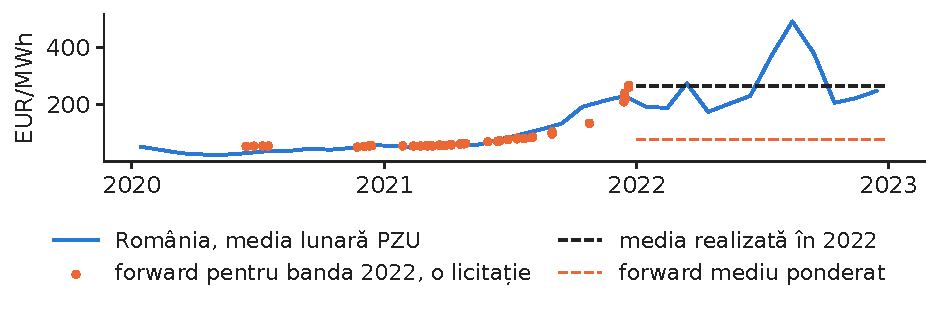
\includegraphics[width=\textwidth,height=0.474\textheight,keepaspectratio]{charts/ro/crisis_cal22.pdf}\end{center}\vspace{-3mm}
\chartsource{Sursa: OPCOM (rezultatele PCCB-LE-flex; prețuri PZU, prin energy-charts.info); BCE. Date: 150 de licitații pentru banda 2022; spot 2020-2022.}
\vspace{0.5mm}
\begin{itemize}\setlength{\itemsep}{0pt}
  \item Banda pentru 2022: 150 de licitații, preț mediu ponderat cu volumul (VWAP) 77{,}4 EUR/MWh; spot 265{,}3
    \begin{itemize}\setlength{\itemsep}{0pt}
      \item VWAP: 2020 -- 54{,}4; sem.\ I 2021 -- 61{,}5; sem.\ II 2021 -- 136{,}7; economie: 1{,}65 mil.\ EUR/MW
    \end{itemize}
\end{itemize}
\par\vfill\manager{contează și momentul: contractele cumpărate la sfîrșitul lui 2021 au costat dublu.}\par\vspace{0.5mm}
\par\vfill\noindent{\scriptsize\color{FooterGray}(calcule proprii; OPCOM)}\hfill\qlink{EMQA\_L5\_crisis\_cal22}{Quantlets/L5/EMQA_L5_crisis_cal22}\par\vspace{0.5mm}
\end{frame}

\begin{frame}{Criza a blocat piața forward și a adus prețuri reglementate}
\footnotesize
\begin{itemize}\setlength{\itemsep}{1pt}
  \item \textbf{Un transfer, nu un cîștig}
    \begin{itemize}\setlength{\itemsep}{0pt}
      \item Fiecare MWh vîndut forward pentru 2022 a fost cu 187{,}9 EUR/MWh sub spot: producătorii au pierdut exact cît au economisit furnizorii acoperiți
    \end{itemize}
  \item \textbf{Apoi prețurile forward au crescut excesiv}
    \begin{itemize}\setlength{\itemsep}{0pt}
      \item Banda pentru 2023 s-a tranzacționat la 509{,}2 EUR/MWh la 17 august 2022; media realizată în 2023: 103{,}7
    \end{itemize}
  \item \textbf{În România}
    \begin{itemize}\setlength{\itemsep}{0pt}
      \item Ordonanța de urgență a Guvernului (OUG) 27/2022: prețuri finale plafonate
      \item OUG 153/2022: Mecanismul de achiziție centralizată de energie electrică (MACEE), cu OPCOM cumpărător unic la 450 lei/MWh, în 2023--2024
      \item Volumul forward pe OPCOM: 27{,}3 TWh în 2021, doar 1{,}6 TWh în 2023
    \end{itemize}
  \item \textbf{În UE}
    \begin{itemize}\setlength{\itemsep}{0pt}
      \item Agenția UE pentru Cooperarea Autorităților de Reglementare din Domeniul Energiei (ACER) a păstrat modelul pieței și a semnalat lichiditatea redusă a contractelor forward pe peste trei ani
    \end{itemize}
\end{itemize}
\par\vfill\manager{scrieți politica de acoperire înainte de criză
    \begin{itemize}\setlength{\itemsep}{0pt}
      \item În timpul crizei, nimeni nu mai cade de acord asupra ei.
    \end{itemize}}\par\vspace{0.5mm}
\par\vfill\noindent{\scriptsize\color{FooterGray}(OUG 27/2022; OUG 153/2022; ACER, 2022; OPCOM)}\hfill\tryit{notebook-ul Jupyter, secțiunea 2}\par\vspace{0.5mm}
\end{frame}


\section{Contracte forward, futures și curba forward}

\subsection{Contractele}

\begin{frame}{Un forward pe energie livrează aceeași putere pe toată perioada}
\footnotesize
\intuition{Un forward în bandă fixează azi prețul tuturor orelor dintr-o lună, un trimestru sau un an.}
\begin{columns}[T,onlytextwidth]
\begin{column}{0.53\textwidth}
\[ \bar S=\frac{1}{H}\sum_{h=1}^{H}S_h,\qquad \underbrace{V_T=q\,H\,(\bar S-F)}_{\text{valoarea pentru cumpărător}} \]{\footnotesize\begin{itemize}\setlength{\itemsep}{0pt}
  \item \textbf{\txtwhere}
    \begin{itemize}\setlength{\itemsep}{0pt}
      \item $H$ = orele perioadei de livrare (744 într-o lună de 31 de zile, 8\,760 într-un an)
      \item $S_h$ = prețul PZU al orei $h$
      \item $q$ = puterea, în MW
      \item $F$ = prețul forward.
    \end{itemize}
\end{itemize}\par}
\end{column}
\begin{column}{0.44\textwidth}
\begin{itemize}\setlength{\itemsep}{1pt}
  \item \textbf{Profiluri}
    \begin{itemize}\setlength{\itemsep}{0pt}
      \item Bandă: toate orele, luni--duminică (LD), 94\% din volum
      \item Vîrf: numai orele de vîrf ale zilelor lucrătoare
    \end{itemize}
  \item \textbf{OPCOM, 31 octombrie 2026}
    \begin{itemize}\setlength{\itemsep}{0pt}
      \item Anul 2027: 148{,}1 EUR/MWh, pentru 8\,760 MWh pe MW
      \item Luna următoare: 215{,}3 EUR/MWh
    \end{itemize}
\end{itemize}
\end{column}
\end{columns}
\par\vfill\manager{faceți oferta către client pe baza prețului forward al perioadei de livrare, nu a prețului spot de azi.}\par\vspace{0.5mm}
\par\vfill\noindent{\scriptsize\color{FooterGray}(OPCOM; Benth et al., 2008)}\hfill\tryit{notebook-ul Jupyter, secțiunea 3}\par\vspace{0.5mm}
\end{frame}

\begin{frame}{Livrarea fizică și decontarea financiară}
\footnotesize
\intuition{Forward-ul fizic livrează energia la prețul $F$; contractul futures financiar plătește doar diferența față de o medie.}
\begin{columns}[T,onlytextwidth]
\begin{column}{0.55\textwidth}
\[ \underbrace{F\cdot Q}_{\text{fizic}}=\underbrace{\bar S Q}_{\text{spot}}-\underbrace{(\bar S^{\text{ref}}-F)Q}_{\text{decontare}}\ \text{numai dacă } \bar S^{\text{ref}}=\bar S \]{\footnotesize\begin{itemize}\setlength{\itemsep}{0pt}
  \item \textbf{\txtwhere}
    \begin{itemize}\setlength{\itemsep}{0pt}
      \item $\bar S^{\text{ref}}$ = indicele de decontare (de exemplu, media din Germania)
      \item Altfel, diferența este riscul de bază (secțiunea 4).
    \end{itemize}
\end{itemize}\par}
\end{column}
\begin{column}{0.42\textwidth}
\begin{itemize}\setlength{\itemsep}{1pt}
  \item \textbf{Fizic, în România}
    \begin{itemize}\setlength{\itemsep}{0pt}
      \item Licitațiile OPCOM PCCB-LE și piața centralizată cu negociere continuă (PC-OTC)
      \item Fără risc de bază
    \end{itemize}
  \item \textbf{Financiar, în străinătate}
    \begin{itemize}\setlength{\itemsep}{0pt}
      \item Contracte futures EEX și HUDEX, cu casă de compensație
      \item În locul riscului de contrapartidă apare nevoia de lichiditate pentru marjă
    \end{itemize}
\end{itemize}
\end{column}
\end{columns}
\par\vfill\manager{contracte fizice, pentru energie livrată în România
    \begin{itemize}\setlength{\itemsep}{0pt}
      \item Contracte financiare, pentru o piață lichidă, cu riscul de bază asumat.
    \end{itemize}}\par\vspace{0.5mm}
\par\vfill\noindent{\scriptsize\color{FooterGray}(OPCOM; Hull, 2022)}\par\vspace{0.5mm}
\end{frame}

\begin{frame}{Contractele futures se decontează zilnic, deci cer lichiditate}
\footnotesize
\intuition{Forward-ul se decontează o dată, la livrare; deținătorul unui contract futures plătește sau încasează zilnic variația prețului.}
\begin{columns}[T,onlytextwidth]
\begin{column}{0.54\textwidth}
\[ \underbrace{VM_t=Q(F_t-F_{t-1})}_{\text{marja de variație}},\qquad \sum_{t=1}^{T}VM_t=Q(F_T-F_0) \]{\footnotesize\begin{itemize}\setlength{\itemsep}{0pt}
  \item \textbf{\txtwhere}
    \begin{itemize}\setlength{\itemsep}{0pt}
      \item $F_t$ = prețul de decontare din ziua $t$
      \item $Q$ = poziția, în MWh
      \item Marja inițială se calculează cu un model de valoare expusă la risc (VaR), vezi cursul 4.
    \end{itemize}
\end{itemize}\par}
\end{column}
\begin{column}{0.43\textwidth}
\begin{itemize}\setlength{\itemsep}{1pt}
  \item \textbf{NYMEX TTF, decembrie 2026}
    \begin{itemize}\setlength{\itemsep}{0pt}
      \item 1\,487 de prețuri zilnice, între 15{,}1 și 103{,}9 EUR/MWh
      \item Cea mai mare variație zilnică: 11{,}83 EUR/MWh, la 29 august 2022
      \item 10 MW $\times$ 744 h: apel în marjă de 88\,015 EUR într-o zi
    \end{itemize}
\end{itemize}
\end{column}
\end{columns}
\par\vfill\manager{dimensionați linia de credit pentru cea mai mare variație zilnică înainte de a vă acoperi la bursă.}\par\vspace{0.5mm}
\par\vfill\noindent{\scriptsize\color{FooterGray}(calcule proprii; Hull, 2022)}\hfill\tryit{notebook-ul Jupyter, secțiunea 3}\par\vspace{0.5mm}
\end{frame}

\begin{frame}{Volumul forward din România s-a prăbușit în 2022--2023}
\small
\begin{center}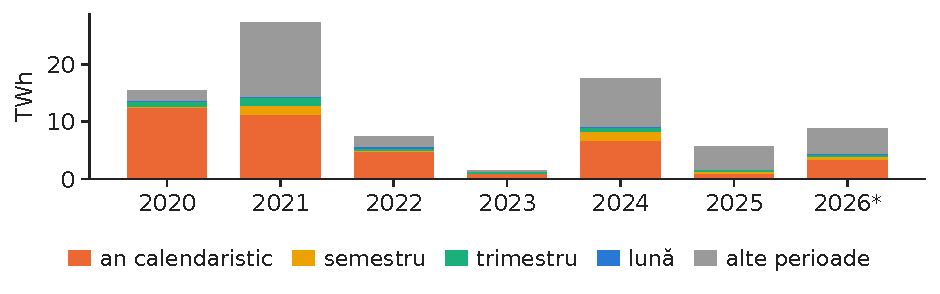
\includegraphics[width=\textwidth,height=0.476\textheight,keepaspectratio]{charts/ro/fw_volume.pdf}\end{center}\vspace{-3mm}
\chartsource{Sursa: OPCOM, rezultatele PCCB-LE-flex; BCE (EUR/RON). Date: 2\,298 de licitații încheiate, 2020-05-12 - 2026-10-31; *2026 pînă la data-limită.}
\vspace{0.5mm}
\begin{itemize}\setlength{\itemsep}{0pt}
  \item Trei producători vînd 83\% din volum: Complexul Energetic Oltenia 32\%, Nuclearelectrica 30\%, Hidroelectrica 21\%
    \begin{itemize}\setlength{\itemsep}{0pt}
      \item Produsele pe an calendaristic: 80\% din volumul în bandă
    \end{itemize}
\end{itemize}
\par\vfill\manager{lichiditatea este redusă: eșalonați cumpărările pe mai multe licitații.}\par\vspace{0.5mm}
\par\vfill\noindent{\scriptsize\color{FooterGray}(calcule proprii; OPCOM)}\hfill\qlink{EMQA\_L5\_fw\_volume}{Quantlets/L5/EMQA_L5_fw_volume}\par\vspace{0.5mm}
\end{frame}

\subsection{Curba prețurilor forward}

\begin{frame}{Forward-ul gazelor reflectă costul de stocare; al energiei, nu}
\footnotesize
\intuition{Gazele se pot stoca, deci prețul lor forward este legat de spot prin costul de deținere; energia electrică nu, deci prețul ei forward este prețul spot așteptat plus o primă de risc.}
\begin{columns}[T,onlytextwidth]
\begin{column}{0.52\textwidth}
\[ \underbrace{F_{t,T}=S_te^{(r+u-y)(T-t)}}_{\text{stocabil}},\qquad \underbrace{F_{t,T}=\E_t[\bar S_T]+\pi_{t,T}}_{\text{energie}} \]{\footnotesize\begin{itemize}\setlength{\itemsep}{0pt}
  \item \textbf{\txtwhere}
    \begin{itemize}\setlength{\itemsep}{0pt}
      \item $r$ = dobînda
      \item $u$ = costul de stocare
      \item $y$ = randamentul de comoditate (convenience yield)
      \item $\pi$ = prima de risc
      \item Report (contango): $F>S$
      \item Deport (backwardation): $F<S$.
    \end{itemize}
\end{itemize}\par}
\end{column}
\begin{column}{0.45\textwidth}
\begin{itemize}\setlength{\itemsep}{1pt}
  \item \textbf{Gaze}, NYMEX TTF, 30 octombrie 2026
    \begin{itemize}\setlength{\itemsep}{0pt}
      \item Decembrie 2026: 103{,}9; mai 2027: 78{,}1 EUR/MWh
      \item Diferența dintre prețul de iarnă și cel de vară acoperă costul stocării
    \end{itemize}
  \item \textbf{Energie electrică}, OPCOM
    \begin{itemize}\setlength{\itemsep}{0pt}
      \item Spot în octombrie: 239{,}3; trimestrul I 2027: 176{,}7; anul 2027: 148{,}1
      \item Deport (backwardation): piața se așteaptă ca prețurile ridicate de acum să scadă
    \end{itemize}
\end{itemize}
\end{column}
\end{columns}
\par\vfill\manager{nu puneți spotul de azi în bugetul anului viitor
    \begin{itemize}\setlength{\itemsep}{0pt}
      \item Folosiți curba forward.
    \end{itemize}}\par\vspace{0.5mm}
\par\vfill\noindent{\scriptsize\color{FooterGray}(Fama \& French, 1987; Bessembinder \& Lemmon, 2002)}\hfill\tryit{notebook-ul Jupyter, secțiunea 3}\par\vspace{0.5mm}
\end{frame}

\begin{frame}{Curba forward din România coboară de la un spot ridicat}
\small
\begin{center}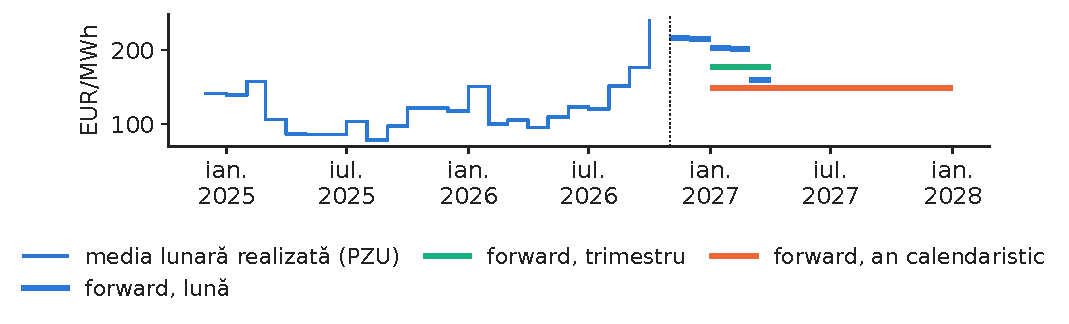
\includegraphics[width=\textwidth,height=0.531\textheight,keepaspectratio]{charts/ro/fwd_curve.pdf}\end{center}\vspace{-3mm}
\chartsource{Sursa: OPCOM (rezultatele PCCB-LE-flex; prețuri PZU, prin energy-charts.info); BCE. Date: 85 de licitații, 2026-09-01 - 2026-10-31.}
\vspace{0.5mm}
\begin{itemize}\setlength{\itemsep}{0pt}
  \item 7 produse în bandă, VWAP pe perioada de livrare: luna următoare 215{,}3, trimestrul I 176{,}7, anul 2027 148{,}1 EUR/MWh.
\end{itemize}
\par\vfill\manager{o ofertă pentru 2027 pornește de la 148 EUR/MWh, nu de la spotul din octombrie.}\par\vspace{0.5mm}
\par\vfill\noindent{\scriptsize\color{FooterGray}(calcule proprii; OPCOM)}\hfill\qlink{EMQA\_L5\_fwd\_curve}{Quantlets/L5/EMQA_L5_fwd_curve}\par\vspace{0.5mm}
\end{frame}

\begin{frame}{Curba se mișcă: prețurile anuale, după data tranzacției}
\small
\begin{center}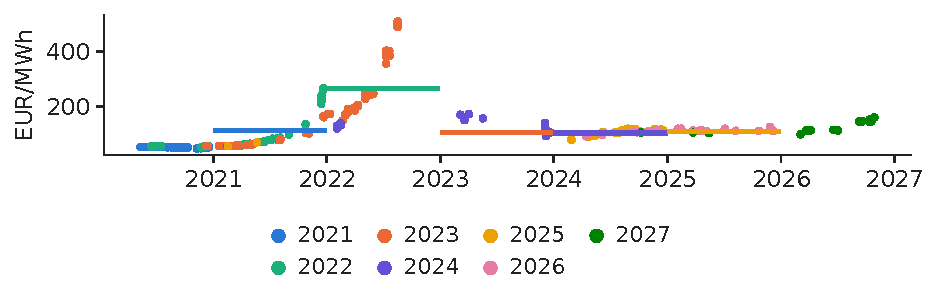
\includegraphics[width=\textwidth,height=0.477\textheight,keepaspectratio]{charts/ro/cal_by_trade.pdf}\end{center}\vspace{-3mm}
\chartsource{Sursa: OPCOM (rezultatele PCCB-LE-flex; prețuri PZU, prin energy-charts.info); BCE. Date: licitații pentru ani calendaristici, pînă la 2026-10-31; linia groasă = media realizată.}
\vspace{0.5mm}
\begin{itemize}\setlength{\itemsep}{0pt}
  \item 2021: VWAP 51{,}3, realizat 111{,}4
    \begin{itemize}\setlength{\itemsep}{0pt}
      \item 2023: 172{,}5 față de 103{,}7
      \item 2025: 102{,}1 față de 108{,}2 EUR/MWh.
    \end{itemize}
\end{itemize}
\par\vfill\manager{prețul forward este prețul certitudinii, nu o prognoză pentru vremuri de criză.}\par\vspace{0.5mm}
\par\vfill\noindent{\scriptsize\color{FooterGray}(calcule proprii; OPCOM)}\hfill\qlink{EMQA\_L5\_cal\_by\_trade}{Quantlets/L5/EMQA_L5_cal_by_trade}\par\vspace{0.5mm}
\end{frame}

\begin{frame}{Prima forward ex post nu are un semn stabil în România}
\footnotesize
\intuition{Dacă cumpărătorii se tem de salturi mai mult decît vînzătorii de scăderi, forward-ul depășește spotul așteptat.}
\begin{columns}[T,onlytextwidth]
\begin{column}{0.50\textwidth}
\[ \hat\pi_i=F_i-\bar S_i,\qquad t=\frac{\bar\pi}{\widehat{\text{se}}_{\text{HAC}}(\bar\pi)} \]{\footnotesize\begin{itemize}\setlength{\itemsep}{0pt}
  \item \textbf{\txtwhere}
    \begin{itemize}\setlength{\itemsep}{0pt}
      \item $i$ = luna de livrare
      \item $F_i$ = VWAP al benzii lunare cumpărate în luna anterioară
      \item $\bar S_i$ = media realizată
      \item Eroare standard robustă la heteroscedasticitate și autocorelare (HAC), Newey--West, 3 decalaje.
    \end{itemize}
\end{itemize}\par}
\end{column}
\begin{column}{0.47\textwidth}
\begin{itemize}\setlength{\itemsep}{1pt}
  \item \textbf{Cu o lună înainte}, 30 de luni
    \begin{itemize}\setlength{\itemsep}{0pt}
      \item Media \ensuremath{+}5{,}2 EUR/MWh, $t$ = 0{,}42, $p$ = 0{,}68
      \item Din 2023: \ensuremath{+}24{,}5, $t$ = 1{,}51
    \end{itemize}
  \item \textbf{Toate produsele}, ponderate cu volumul
    \begin{itemize}\setlength{\itemsep}{0pt}
      \item Livrate pînă în 2021: \ensuremath{-}55{,}8
      \item 2022: \ensuremath{-}166{,}5; din 2023: \ensuremath{+}29{,}7 EUR/MWh
    \end{itemize}
\end{itemize}
\end{column}
\end{columns}
\par\vfill\manager{acoperirea este, în medie, ieftină
    \begin{itemize}\setlength{\itemsep}{0pt}
      \item Costul ei real este cîștigul la care renunțați.
    \end{itemize}}\par\vspace{0.5mm}
\par\vfill\noindent{\scriptsize\color{FooterGray}(Bessembinder \& Lemmon, 2002; Redl et al., 2009)}\hfill\tryit{notebook-ul Jupyter, secțiunea 3}\par\vspace{0.5mm}
\end{frame}

\begin{frame}{Lună de lună, diferența forward minus spot are ambele semne}
\small
\begin{center}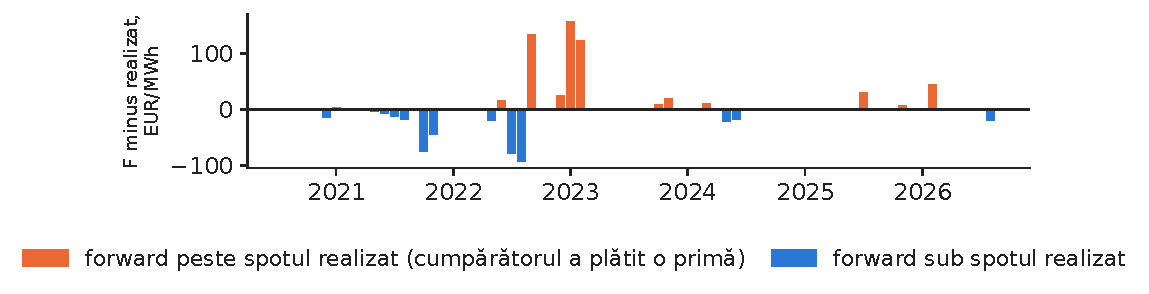
\includegraphics[width=\textwidth,height=0.556\textheight,keepaspectratio]{charts/ro/premium.pdf}\end{center}\vspace{-3mm}
\chartsource{Sursa: OPCOM (rezultatele PCCB-LE-flex; prețuri PZU, prin energy-charts.info); BCE. Date: 30 de luni de livrare, 2020-08 - 2026-08.}
\vspace{0.5mm}
\begin{itemize}\setlength{\itemsep}{0pt}
  \item Mediana: \ensuremath{-}0{,}2 EUR/MWh
    \begin{itemize}\setlength{\itemsep}{0pt}
      \item Valorile negative mari reflectă creșterile neașteptate de preț din 2021--2022, nu o primă negativă sistematică.
    \end{itemize}
\end{itemize}
\par\vfill\manager{judecați o acoperire după riscul eliminat, nu după profitul de după livrare.}\par\vspace{0.5mm}
\par\vfill\noindent{\scriptsize\color{FooterGray}(calcule proprii; OPCOM)}\hfill\qlink{EMQA\_L5\_premium}{Quantlets/L5/EMQA_L5_premium}\par\vspace{0.5mm}
\end{frame}


\section{Marjele centralelor electrice}

\begin{frame}{Clean spark spread: energie minus gaze minus carbon}
\footnotesize
\intuition{O centrală pe gaze vinde 1 MWh, arde $1/\eta$ MWh de gaze și plătește certificatele pentru CO$_2$ emis.}
\begin{columns}[T,onlytextwidth]
\begin{column}{0.55\textwidth}
\[ SS=P-\frac{G}{\eta_g},\qquad CSS=P-\frac{G}{\eta_g}-\frac{e_g}{\eta_g}A \]{\footnotesize\begin{itemize}\setlength{\itemsep}{0pt}
  \item \textbf{\txtwhere}
    \begin{itemize}\setlength{\itemsep}{0pt}
      \item Spark spread (SS), clean spark spread (CSS)
      \item $P$ = prețul energiei electrice, EUR/MWh
      \item $G$ = prețul gazelor, EUR/MWh termic
      \item $\eta_g$ = randamentul centralei pe gaze, 0{,}50 (ipoteză)
      \item $e_g$ = factorul de emisie al gazelor, 0{,}202 t CO$_2$/MWh termic, Grupul interguvernamental privind schimbările climatice (IPCC)
      \item $A$ = prețul EUA, EUR/t.
    \end{itemize}
\end{itemize}\par}
\end{column}
\begin{column}{0.42\textwidth}
\begin{itemize}\setlength{\itemsep}{1pt}
  \item \textbf{România, octombrie 2026}
    \begin{itemize}\setlength{\itemsep}{0pt}
      \item Prețul energiei 239{,}3; costul gazelor pe MWh electric 173{,}6 (= 86{,}8/0,5); costul carbonului 33{,}3 EUR/MWh
      \item SS \ensuremath{+}65{,}7, CSS \ensuremath{+}32{,}4 EUR/MWh
    \end{itemize}
  \item \textbf{CSS, media anuală}
    \begin{itemize}\setlength{\itemsep}{0pt}
      \item România: 2022 \ensuremath{-}32{,}2, 2025 \ensuremath{+}5{,}8
      \item Germania: 2022 \ensuremath{-}62{,}2, 2025 \ensuremath{-}13{,}1
    \end{itemize}
\end{itemize}
\end{column}
\end{columns}
\par\vfill\manager{producătorul pe gaze acoperă marja: vinde energie și cumpără gaze și EUA forward, simultan.}\par\vspace{0.5mm}
\par\vfill\noindent{\scriptsize\color{FooterGray}(IPCC, 2006; Deng et al., 2001)}\hfill\tryit{notebook-ul Jupyter, secțiunea 4}\par\vspace{0.5mm}
\end{frame}

\begin{frame}{Dark spread și prețul carbonului care favorizează gazele}
\footnotesize
\intuition{Cărbunele emite mai mult CO$_2$ pe MWh, deci un EUA scump împinge cărbunele după gaze în ordinea de merit.}
\begin{columns}[T,onlytextwidth]
\begin{column}{0.56\textwidth}
\[ CDS=P-\frac{C}{\eta_c}-\frac{e_c}{\eta_c}A,\qquad A^{*}=\frac{G/\eta_g-C/\eta_c}{e_c/\eta_c-e_g/\eta_g} \]{\footnotesize\begin{itemize}\setlength{\itemsep}{0pt}
  \item \textbf{\txtwhere}
    \begin{itemize}\setlength{\itemsep}{0pt}
      \item Clean dark spread (CDS)
      \item $C$ = prețul cărbunelui, EUR/MWh termic (USD/t $\div$ EUR/USD $\div$ 6{,}978)
      \item $\eta_c$ = randamentul centralei pe cărbune, 0{,}38 (ipoteză)
      \item $e_c$ = factorul de emisie, 0{,}341 t CO$_2$/MWh termic
      \item $A^{*}$ = prețul EUA la care CSS = CDS.
    \end{itemize}
\end{itemize}\par}
\end{column}
\begin{column}{0.41\textwidth}
\begin{itemize}\setlength{\itemsep}{1pt}
  \item \textbf{Luna: octombrie 2026}
    \begin{itemize}\setlength{\itemsep}{0pt}
      \item Cărbune 12{,}8 EUR/MWh termic; CDS în România \ensuremath{+}131{,}7
      \item $A^{*}$ = 283{,}7 EUR/t, față de EUA 82{,}4
    \end{itemize}
  \item \textbf{Limite}
    \begin{itemize}\setlength{\itemsep}{0pt}
      \item Lignitul nu are preț de piață; folosim cărbunele sud-african de export
      \item EUA = licitațiile EEX, apoi titlul ETC din ianuarie 2026
    \end{itemize}
\end{itemize}
\end{column}
\end{columns}
\par\vfill\manager{producătorul pe cărbune care vinde energie forward trebuie să cumpere și EUA forward.}\par\vspace{0.5mm}
\par\vfill\noindent{\scriptsize\color{FooterGray}(IPCC, 2006; World Bank)}\hfill\tryit{notebook-ul Jupyter, secțiunea 4}\par\vspace{0.5mm}
\end{frame}

\begin{frame}{Clean spark spread și clean dark spread, lunar}
\small
\begin{center}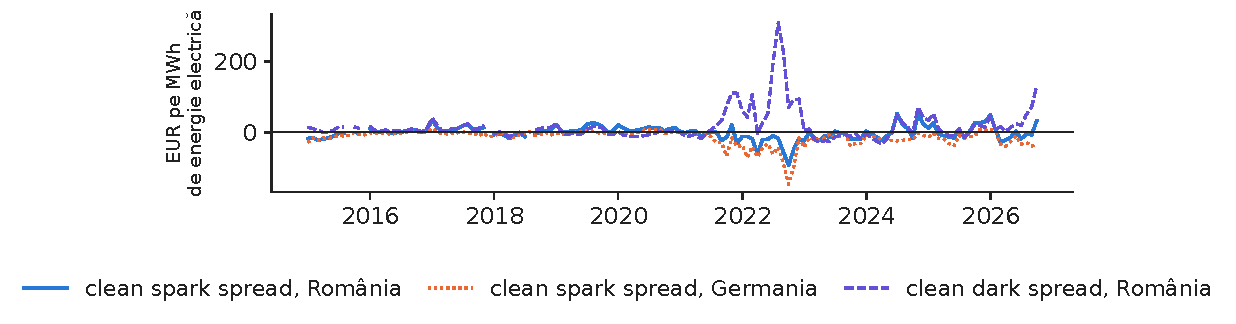
\includegraphics[width=\textwidth,height=0.555\textheight,keepaspectratio]{charts/ro/spreads.pdf}\end{center}\vspace{-3mm}
\chartsource{Sursa: energy-charts.info; Banca Mondială (TTF, cărbune); EEX și SparkChange ETC (EUA); BCE. Date: lunar, 2015-01 - 2026-10.}
\vspace{0.5mm}
\begin{itemize}\setlength{\itemsep}{0pt}
  \item CSS negativ în 67 din 138 de luni în România și în 121 în Germania
    \begin{itemize}\setlength{\itemsep}{0pt}
      \item În medie, cu 13{,}9 EUR/MWh mai mare în România.
    \end{itemize}
\end{itemize}
\par\vfill\manager{o marjă medie apropiată de zero nu face centrala inutilă: ea funcționează doar în orele bune.}\par\vspace{0.5mm}
\par\vfill\noindent{\scriptsize\color{FooterGray}(calcule proprii; IPCC, 2006)}\hfill\qlink{EMQA\_L5\_spreads}{Quantlets/L5/EMQA_L5_spreads}\par\vspace{0.5mm}
\end{frame}

\begin{frame}{O centrală pe gaze flexibilă este o serie de opțiuni call orare}
\footnotesize
\intuition{Centrala funcționează doar cînd marja este pozitivă, deci încasează partea pozitivă a fiecărei marje orare.}
\begin{columns}[T,onlytextwidth]
\begin{column}{0.52\textwidth}
\[ \underbrace{\sum_h \max(CSS_h,0)}_{\text{flexibilă}}\ \ge\ \max\Big(\underbrace{\sum_h CSS_h}_{\text{continuă}},0\Big) \]{\footnotesize\begin{itemize}\setlength{\itemsep}{0pt}
  \item \textbf{\txtwhere}
    \begin{itemize}\setlength{\itemsep}{0pt}
      \item $CSS_h$ = clean spark spread al orei $h$, pentru 1 MW, cu gaze și EUA la media lunii
      \item Fără costuri de pornire, deci o limită superioară.
    \end{itemize}
\end{itemize}\par}
\end{column}
\begin{column}{0.45\textwidth}
\begin{itemize}\setlength{\itemsep}{1pt}
  \item \textbf{România}, ultimele 12 luni
    \begin{itemize}\setlength{\itemsep}{0pt}
      \item Marjă pozitivă în 58\% din ore
      \item Continuă: 38\,095; flexibilă: 235\,494 EUR pe MW
    \end{itemize}
  \item \textbf{Germania}
    \begin{itemize}\setlength{\itemsep}{0pt}
      \item Marjă pozitivă în 41\% din ore
      \item Continuă: \ensuremath{-}165\,206; flexibilă: 112\,724 EUR pe MW
    \end{itemize}
\end{itemize}
\end{column}
\end{columns}
\par\vfill\manager{evaluați o centrală pe gaze sau o baterie ca opțiuni, nu ca marjă medie înmulțită cu 8\,760 h.}\par\vspace{0.5mm}
\par\vfill\noindent{\scriptsize\color{FooterGray}(Deng et al., 2001; Eydeland \& Wolyniec, 2003)}\hfill\tryit{notebook-ul Jupyter, secțiunea 4}\par\vspace{0.5mm}
\end{frame}

\begin{frame}{Marjele orare ordonate: valoarea stă în orele cele mai bune}
\small
\begin{center}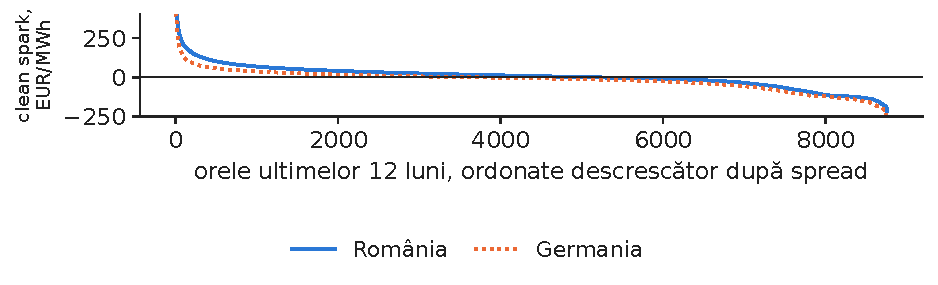
\includegraphics[width=\textwidth,height=0.521\textheight,keepaspectratio]{charts/ro/spark_hourly.pdf}\end{center}\vspace{-3mm}
\chartsource{Sursa: energy-charts.info; Banca Mondială (TTF, cărbune); EEX și SparkChange ETC (EUA); BCE. Date: 2025-11-01 - 2026-10-31, date orare.}
\vspace{0.5mm}
\begin{itemize}\setlength{\itemsep}{0pt}
  \item Aria de deasupra lui zero este valoarea opțiunii
    \begin{itemize}\setlength{\itemsep}{0pt}
      \item La aceleași prețuri ale gazelor și carbonului, România are mai multe ore profitabile decît Germania.
    \end{itemize}
\end{itemize}
\par\vfill\manager{acoperiți o centrală flexibilă cu produse de vîrf, nu cu bandă.}\par\vspace{0.5mm}
\par\vfill\noindent{\scriptsize\color{FooterGray}(calcule proprii)}\hfill\qlink{EMQA\_L5\_spark\_hourly}{Quantlets/L5/EMQA_L5_spark_hourly}\par\vspace{0.5mm}
\end{frame}


\section{Raportul de acoperire, riscul de bază și riscul de profil}

\begin{frame}{Raportul de acoperire optim este panta unei regresii}
\footnotesize
\intuition{Alegem numărul de contracte pe MWh expus care face costul acoperit cît mai stabil.}
\begin{columns}[T,onlytextwidth]
\begin{column}{0.58\textwidth}
\[ h^{*}=\arg\min_h\Var(\Delta S-h\Delta F)=\rho\frac{\sigma_S}{\sigma_F}=\frac{\Cov(\Delta S,\Delta F)}{\Var(\Delta F)} \]\[ \Delta S_t=a+h\,\Delta F_t+\varepsilon_t,\qquad HE=\rho^2 \]{\footnotesize\begin{itemize}\setlength{\itemsep}{0pt}
  \item \textbf{\txtwhere}
    \begin{itemize}\setlength{\itemsep}{0pt}
      \item $\Delta S$, $\Delta F$ = variațiile lunare ale expunerii și ale instrumentului
      \item $\rho$ = corelația lor
      \item Eficiența acoperirii (HE) = varianța eliminată
      \item $h^{*}$ prin metoda celor mai mici pătrate (OLS)
      \item Demonstrația în anexa A.
    \end{itemize}
\end{itemize}\par}
\end{column}
\begin{column}{0.39\textwidth}
\begin{itemize}\setlength{\itemsep}{1pt}
  \item \textbf{Instrumentul}
    \begin{itemize}\setlength{\itemsep}{0pt}
      \item Un contract futures financiar ajunge la media lunară a zonei sale: folosim mediile HU și DE-LU
      \item 133 de luni, februarie 2015 -- octombrie 2026
    \end{itemize}
  \item \textbf{Incertitudinea}
    \begin{itemize}\setlength{\itemsep}{0pt}
      \item Eroare standard HAC, 3 decalaje
      \item Bootstrap pe blocuri de 6 luni, 2\,000 de replicări
    \end{itemize}
\end{itemize}
\end{column}
\end{columns}
\par\vfill\manager{un raport de acoperire fără interval de încredere este o simplă presupunere.}\par\vspace{0.5mm}
\par\vfill\noindent{\scriptsize\color{FooterGray}(Johnson, 1960; Ederington, 1979)}\hfill\tryit{notebook-ul Jupyter, secțiunea 5}\par\vspace{0.5mm}
\end{frame}

\begin{frame}{Contractele din Ungaria acoperă aproape tot riscul; cele germane lasă o cincime}
\footnotesize
\begin{center}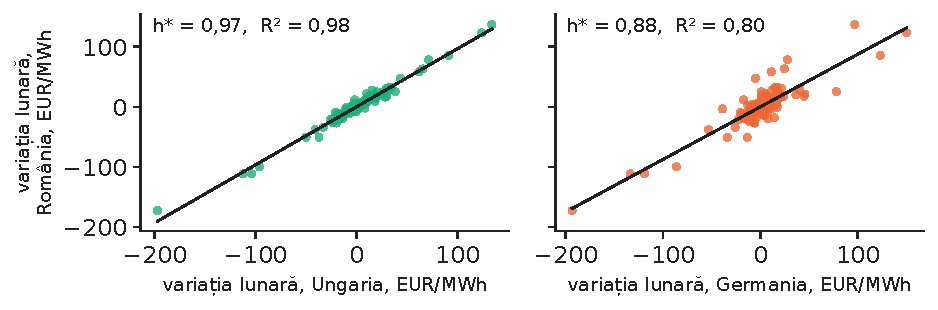
\includegraphics[width=\textwidth,height=0.441\textheight,keepaspectratio]{charts/ro/hedge_scatter.pdf}\end{center}\vspace{-3mm}
\chartsource{Sursa: energy-charts.info: prețurile PZU ale OPCOM, HUPX, EPEX SPOT. Date: variații lunare, 2015-02 - 2026-10.}
\vspace{0.3mm}
\begin{center}{\scriptsize\renewcommand{\arraystretch}{1.05}\setlength{\tabcolsep}{4pt}
\begin{tabular}{@{}lrrrrrr@{}}\toprule
Instrument & $h^{*}$ & eroare std.\ HAC & bootstrap 95\% & $R^2$ & $h^{*}$ 2015--20 & varianță eliminată, din 2021 \\ \midrule
Ungaria & 0{,}966 & 0{,}023 & [0{,}93; 1{,}03] & 0{,}98 & 0{,}92 & 97{,}9\% \\
Germania & 0{,}875 & 0{,}049 & [0{,}73; 1{,}01] & 0{,}80 & 0{,}91 & 81{,}1\% \\
\bottomrule\end{tabular}}\end{center}
\par\vfill\manager{folosiți contractele din Ungaria înaintea celor din Germania.}\par\vspace{0.5mm}
\par\vfill\noindent{\scriptsize\color{FooterGray}(calcule proprii; $h^{*}$ din 2015--2020, testat din 2021)}\hfill\qlink{EMQA\_L5\_hedge\_scatter}{Quantlets/L5/EMQA_L5_hedge_scatter}\par\vspace{0.5mm}
\end{frame}

\begin{frame}{Riscul de bază: ce lasă descoperit un contract din altă zonă}
\footnotesize
\intuition{Acoperit cu un contract futures german, furnizorul din România plătește forward-ul german plus diferența România--Germania de la livrare.}
\begin{columns}[T,onlytextwidth]
\begin{column}{0.55\textwidth}
\[ \bar S^{\text{RO}}-h(\bar S^{X}-F^{X}_0)=hF^{X}_0+\underbrace{(\bar S^{\text{RO}}-h\bar S^{X})}_{\text{baza } b} \]{\footnotesize\begin{itemize}\setlength{\itemsep}{0pt}
  \item \textbf{\txtwhere}
    \begin{itemize}\setlength{\itemsep}{0pt}
      \item $X$ = zona contractului (HU, DE-LU)
      \item $F^{X}_0$ = prețul lui de azi
      \item Pentru $h=1$, $b$ = diferența lunară de preț România minus $X$.
    \end{itemize}
\end{itemize}\par}
\end{column}
\begin{column}{0.42\textwidth}
\begin{itemize}\setlength{\itemsep}{1pt}
  \item \textbf{România -- Ungaria}
    \begin{itemize}\setlength{\itemsep}{0pt}
      \item Media \ensuremath{-}2{,}1, abaterea standard 4{,}5 EUR/MWh
      \item Prețuri egale în 56\% din ore în 2021
    \end{itemize}
  \item \textbf{România -- Germania}
    \begin{itemize}\setlength{\itemsep}{0pt}
      \item Media \ensuremath{+}13{,}9, abaterea standard 15{,}2
      \item Din 2023, media \ensuremath{+}18{,}7 EUR/MWh
    \end{itemize}
\end{itemize}
\end{column}
\end{columns}
\par\vfill\manager{o acoperire germană costă forward-ul german plus circa 19 EUR/MWh: includeți diferența în ofertă.}\par\vspace{0.5mm}
\par\vfill\noindent{\scriptsize\color{FooterGray}(Hull, 2022; calcule proprii)}\hfill\tryit{notebook-ul Jupyter, secțiunea 5}\par\vspace{0.5mm}
\end{frame}

\begin{frame}{Volatilitatea bazei a crescut după 2021, deși RO și HU au adesea același preț}
\small
\begin{center}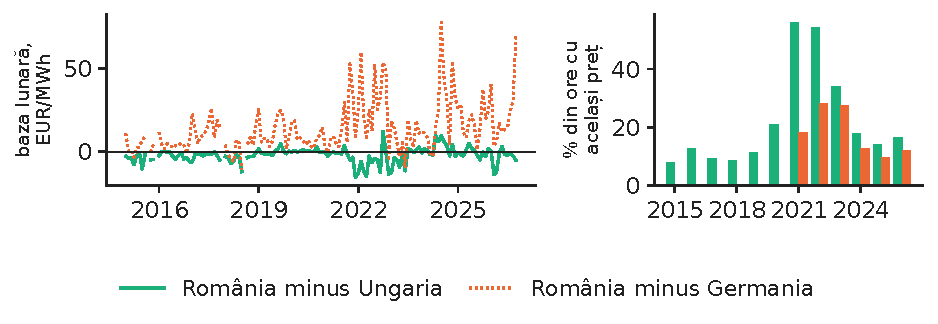
\includegraphics[width=\textwidth,height=0.520\textheight,keepaspectratio]{charts/ro/basis.pdf}\end{center}\vspace{-3mm}
\chartsource{Sursa: energy-charts.info: prețurile PZU ale OPCOM, HUPX, EPEX SPOT. Date: 2015-01 - 2026-10; dreapta: diferență sub 0,01 EUR/MWh.}
\vspace{0.5mm}
\begin{itemize}\setlength{\itemsep}{0pt}
  \item Baza față de Germania: abaterea standard 7{,}6 înainte de 2021 și 18{,}2 după
    \begin{itemize}\setlength{\itemsep}{0pt}
      \item Etape ale cuplării: 17 iunie 2021 (Interim Coupling), 8 iunie 2022 (Core, bazată pe fluxuri).
    \end{itemize}
\end{itemize}
\par\vfill\manager{prețurile se egalizează doar fără congestie: riscul de bază este un risc de congestie.}\par\vspace{0.5mm}
\par\vfill\noindent{\scriptsize\color{FooterGray}(calcule proprii; ENTSO-E, 2021)}\hfill\qlink{EMQA\_L5\_basis}{Quantlets/L5/EMQA_L5_basis}\par\vspace{0.5mm}
\end{frame}

\begin{frame}{Riscul de profil: clienții nu consumă în bandă}
\footnotesize
\intuition{Banda acoperă aceeași putere în fiecare oră; consumul este mai mare în orele scumpe, producția solară în cele ieftine.}
\begin{columns}[T,onlytextwidth]
\begin{column}{0.53\textwidth}
\[ f^{\text{cons}}=\frac{\sum_h L_hP_h}{\bar P\sum_h L_h},\qquad f^{\text{solar}}=\frac{\sum_h Q_hP_h}{\bar P\sum_h Q_h} \]{\footnotesize\begin{itemize}\setlength{\itemsep}{0pt}
  \item \textbf{\txtwhere}
    \begin{itemize}\setlength{\itemsep}{0pt}
      \item $L_h$ = consumul României, $Q_h$ = producția solară în ora $h$
      \item $\bar P$ = media simplă a anului
      \item $f>1$: profilul costă mai mult decît banda.
    \end{itemize}
\end{itemize}\par}
\end{column}
\begin{column}{0.44\textwidth}
\begin{itemize}\setlength{\itemsep}{1pt}
  \item \textbf{Furnizorul}, consumul național
    \begin{itemize}\setlength{\itemsep}{0pt}
      \item $f^{\text{cons}}$: 1{,}039 (2019), 1{,}066 (2025)
      \item +7{,}1 EUR/MWh peste bandă în 2025
    \end{itemize}
  \item \textbf{Producătorul solar}
    \begin{itemize}\setlength{\itemsep}{0pt}
      \item $f^{\text{solar}}$: 1{,}045 (2019), 0{,}596 (2025)
      \item $-$43{,}7 EUR/MWh sub bandă în 2025
    \end{itemize}
\end{itemize}
\end{column}
\end{columns}
\par\vfill\manager{evaluați un contract de achiziție pe termen lung (PPA) pentru un parc solar la raportul de captare ($f^{\text{solar}}$), nu la prețul benzii.}\par\vspace{0.5mm}
\par\vfill\noindent{\scriptsize\color{FooterGray}(calcule proprii)}\hfill\tryit{notebook-ul Jupyter, secțiunea 5}\par\vspace{0.5mm}
\end{frame}

\begin{frame}{Valoarea profilului solar și a profilului de consum față de bandă}
\small
\begin{center}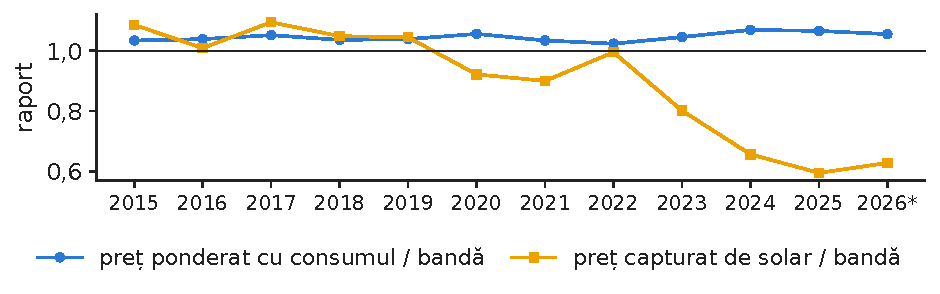
\includegraphics[width=\textwidth,height=0.520\textheight,keepaspectratio]{charts/ro/shape.pdf}\end{center}\vspace{-3mm}
\chartsource{Sursa: energy-charts.info: prețuri OPCOM; consum și producție solară ENTSO-E. Date: date orare, 2015 - 2026-10-31; *pînă la data-limită.}
\vspace{0.5mm}
\begin{itemize}\setlength{\itemsep}{0pt}
  \item Raportul de captare solar a scăzut la 0{,}596 în 2025
    \begin{itemize}\setlength{\itemsep}{0pt}
      \item În 2025, prețul ponderat cu consumul a depășit banda cu 7{,}1 EUR/MWh.
    \end{itemize}
\end{itemize}
\par\vfill\manager{cumpărați bandă pentru baza portofoliului și produse de vîrf sau orare pentru profil.}\par\vspace{0.5mm}
\par\vfill\noindent{\scriptsize\color{FooterGray}(calcule proprii)}\hfill\qlink{EMQA\_L5\_shape}{Quantlets/L5/EMQA_L5_shape}\par\vspace{0.5mm}
\end{frame}


\section{Opțiuni pe energie}

\begin{frame}{Plafon, prag minim și collar}
\footnotesize
\intuition{O opțiune call plafonează prețul de cumpărare și păstrează cîștigul dacă prețurile scad; costă o primă plătită azi.}
\begin{columns}[T,onlytextwidth]
\begin{column}{0.56\textwidth}
\[ \underbrace{(F_T-K)^+}_{\text{call}},\quad \underbrace{(K-F_T)^+}_{\text{put}},\quad \underbrace{\min(F_T,K_c)+c}_{\text{preț cu plafon}} \]\[ \text{collar: } \max\big(K_p,\min(F_T,K_c)\big)+c-p \]{\footnotesize\begin{itemize}\setlength{\itemsep}{0pt}
  \item \textbf{\txtwhere}
    \begin{itemize}\setlength{\itemsep}{0pt}
      \item $F_T$ = prețul forward la scadența $T$
      \item $K$ = prețul de exercitare
      \item $c$, $p$ = primele call și put
      \item Collar = cumpărare call la $K_c$ și vînzare put la $K_p<K_c$.
    \end{itemize}
\end{itemize}\par}
\end{column}
\begin{column}{0.41\textwidth}
\begin{itemize}\setlength{\itemsep}{1pt}
  \item \textbf{Cine ce folosește}
    \begin{itemize}\setlength{\itemsep}{0pt}
      \item Furnizorul: plafon (call)
      \item Producătorul: prag minim (put)
      \item Amîndoi: un collar cu cost redus (furnizorul cumpără call și vinde put; producătorul invers)
    \end{itemize}
  \item \textbf{În România}
    \begin{itemize}\setlength{\itemsep}{0pt}
      \item Nu există opțiuni pe energie listate
      \item Plafoanele apar în contracte bilaterale și PPA
    \end{itemize}
\end{itemize}
\end{column}
\end{columns}
\par\vfill\manager{cumpărați un plafon cînd un salt de preț ar pune firma în pericol, nu doar cînd i-ar reduce profitul.}\par\vspace{0.5mm}
\par\vfill\noindent{\scriptsize\color{FooterGray}(Hull, 2022)}\hfill\tryit{notebook-ul Jupyter, secțiunea 6}\par\vspace{0.5mm}
\end{frame}

\begin{frame}{Modelul Black-76 evaluează o opțiune pe forward cu cinci parametri}
\footnotesize
\intuition{În evaluarea neutră la risc, forward-ul nu are tendință, deci opțiunea depinde doar de $F$, $K$, $T$, $r$ și $\sigma$.}
\begin{columns}[T,onlytextwidth]
\begin{column}{0.58\textwidth}
\[ C=e^{-rT}[F\Phi(d_1)-K\Phi(d_2)],\quad P=e^{-rT}[K\Phi(-d_2)-F\Phi(-d_1)] \]\[ d_1=\frac{\ln(F/K)+\sigma^2T/2}{\sigma\sqrt T},\qquad d_2=d_1-\sigma\sqrt T \]{\footnotesize\begin{itemize}\setlength{\itemsep}{0pt}
  \item \textbf{\txtwhere}
    \begin{itemize}\setlength{\itemsep}{0pt}
      \item $\Phi$ = funcția de repartiție normală standard
      \item $\sigma$ = volatilitatea anuală a lui $\ln F$
      \item $T$ în ani
      \item $r$ = rata dobînzii fără risc, cu capitalizare continuă (anexa B).
    \end{itemize}
\end{itemize}\par}
\end{column}
\begin{column}{0.39\textwidth}
\begin{itemize}\setlength{\itemsep}{1pt}
  \item \textbf{Datele de intrare}, banda pentru 2027
    \begin{itemize}\setlength{\itemsep}{0pt}
      \item $F$ = 148{,}12 EUR/MWh (VWAP OPCOM)
      \item $T$ = 45 de zile; $r$ = 2{,}44\% (€STR)
      \item $\sigma$ = 0{,}220 (diapozitivul următor)
    \end{itemize}
  \item \textbf{Prețuri}, EUR/MWh
    \begin{itemize}\setlength{\itemsep}{0pt}
      \item $K=F$: call = put = 4{,}55
      \item Plafon la 1,1 $F$: 0{,}63
      \item Prag minim la 0,9 $F$: 0{,}43
    \end{itemize}
\end{itemize}
\end{column}
\end{columns}
\par\vfill\manager{întrebați banca ce volatilitate a folosit
    \begin{itemize}\setlength{\itemsep}{0pt}
      \item Prima crește aproape proporțional cu $\sigma$.
    \end{itemize}}\par\vspace{0.5mm}
\par\vfill\noindent{\scriptsize\color{FooterGray}(Black, 1976; Hull, 2022)}\hfill\tryit{notebook-ul Jupyter, secțiunea 6}\par\vspace{0.5mm}
\end{frame}

\begin{frame}{Volatilitatea trebuie estimată, iar estimările reale diferă}
\footnotesize
\begin{columns}[T,onlytextwidth]
\begin{column}{0.55\textwidth}
\begin{itemize}\setlength{\itemsep}{1pt}
  \item \textbf{1. Forward-urile anuale din România}
    \begin{itemize}\setlength{\itemsep}{0pt}
      \item Licitații neregulate: $\hat\sigma^2=\sum_k(\Delta\ln F_k)^2/\sum_k\Delta t_k$, intervale de cel mult 30 de zile
      \item $\hat\sigma$ = 0{,}220, din 49 de perechi de zile cu licitații
    \end{itemize}
  \item \textbf{2. Contractul TTF pentru ianuarie 2027}
    \begin{itemize}\setlength{\itemsep}{0pt}
      \item Ultimele 60 de zile: $\hat\sigma$ = 0{,}499; call 10{,}30
    \end{itemize}
  \item \textbf{3. Media lunară față de forward}
    \begin{itemize}\setlength{\itemsep}{0pt}
      \item $\text{sd}(\ln(\bar S/F)/\sqrt T)$ = 0{,}668, 153 de licitații
    \end{itemize}
\end{itemize}
\end{column}
\begin{column}{0.42\textwidth}
\begin{itemize}\setlength{\itemsep}{1pt}
  \item \textbf{De ce diferă}
    \begin{itemize}\setlength{\itemsep}{0pt}
      \item Un an este media a 8\,760 de ore, mult mai stabilă decît o lună
      \item Gazele trec printr-o criză proprie în 2026
      \item Nu există volatilitate implicită gratuită pentru România
    \end{itemize}
  \item \textbf{Mai bine}
    \begin{itemize}\setlength{\itemsep}{0pt}
      \item Modelele de heteroscedasticitate condiționată autoregresivă generalizată (GARCH) din cursul 3
    \end{itemize}
\end{itemize}
\end{column}
\end{columns}
\par\vfill\manager{alegeți volatilitatea potrivită activului suport: an, trimestru sau lună.}\par\vspace{0.5mm}
\par\vfill\noindent{\scriptsize\color{FooterGray}(calcule proprii; OPCOM; Yahoo Finance)}\hfill\tryit{notebook-ul Jupyter, secțiunea 6}\par\vspace{0.5mm}
\end{frame}

\begin{frame}{Contractele apropiate de livrare variază mai mult: efectul Samuelson}
\small
\begin{center}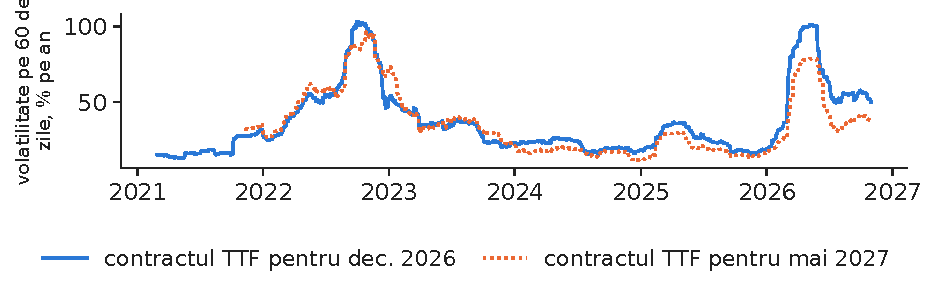
\includegraphics[width=\textwidth,height=0.515\textheight,keepaspectratio]{charts/ro/samuelson.pdf}\end{center}\vspace{-3mm}
\chartsource{Sursa: Yahoo Finance, contracte futures NYMEX TTF. Date: prețuri zilnice pînă la 2026-10-31, fereastră mobilă de 60 de zile.}
\vspace{0.5mm}
\begin{itemize}\setlength{\itemsep}{0pt}
  \item Volatilitatea anualizată, 1 noiembrie 2025 -- 31 octombrie 2026: contractul pentru decembrie 2026 -- 63\%, cel pentru mai 2027 -- 48\%
    \begin{itemize}\setlength{\itemsep}{0pt}
      \item În 2022, ambele în jur de 66\%.
    \end{itemize}
\end{itemize}
\par\vfill\manager{o opțiune apropiată de livrare cere o volatilitate mai mare.}\par\vspace{0.5mm}
\par\vfill\noindent{\scriptsize\color{FooterGray}(calcule proprii; Samuelson, 1965)}\hfill\qlink{EMQA\_L5\_samuelson}{Quantlets/L5/EMQA_L5_samuelson}\par\vspace{0.5mm}
\end{frame}

\begin{frame}{Delta și vega: echivalentul în MWh forward și sensibilitatea la volatilitate}
\footnotesize
\intuition{Delta este cantitatea de forward care compensează opțiunea; vega este variația primei la un punct de volatilitate.}
\begin{columns}[T,onlytextwidth]
\begin{column}{0.52\textwidth}
\[ \Delta_C=e^{-rT}\Phi(d_1),\quad \Delta_P=-e^{-rT}\Phi(-d_1) \]\[ \mathcal V=e^{-rT}F\varphi(d_1)\sqrt T,\qquad C-P=e^{-rT}(F-K) \]{\footnotesize\begin{itemize}\setlength{\itemsep}{0pt}
  \item \textbf{\txtwhere}
    \begin{itemize}\setlength{\itemsep}{0pt}
      \item $\varphi$ = densitatea normală standard
      \item $\mathcal V$ pe un punct de volatilitate (0{,}01)
      \item Ultima relație este paritatea put--call.
    \end{itemize}
\end{itemize}\par}
\end{column}
\begin{column}{0.45\textwidth}
\begin{itemize}\setlength{\itemsep}{1pt}
  \item \textbf{$K=F$}, $\sigma$ = 0{,}220
    \begin{itemize}\setlength{\itemsep}{0pt}
      \item $d_1$ = 0{,}039; $\Delta_C$ = 0{,}514, $\Delta_P$ = \ensuremath{-}0{,}483
      \item Vega 0{,}207 EUR/MWh
      \item $C=P$, cum cere paritatea
    \end{itemize}
  \item \textbf{Plafonul la 1,1 $F$}
    \begin{itemize}\setlength{\itemsep}{0pt}
      \item Delta 0{,}116
      \item Costul plafonului pentru 1 MW pe un an: 5\,519 EUR
    \end{itemize}
\end{itemize}
\end{column}
\end{columns}
\par\vfill\manager{vînzătorul plafonului se acoperă deținînd contracte forward într-o cantitate egală cu delta, pe care o ajustează periodic.}\par\vspace{0.5mm}
\par\vfill\noindent{\scriptsize\color{FooterGray}(Black, 1976; Hull, 2022)}\hfill\tryit{notebook-ul Jupyter, secțiunea 6}\par\vspace{0.5mm}
\end{frame}

\begin{frame}{Prețul efectiv al benzii pentru 2027 cu fiecare instrument}
\small
\begin{center}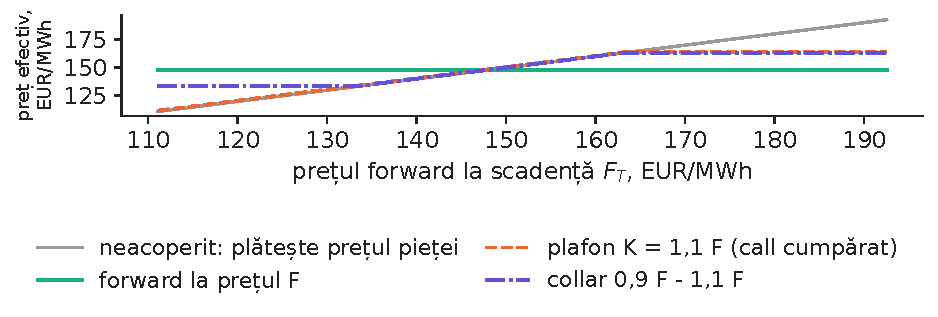
\includegraphics[width=\textwidth,height=0.470\textheight,keepaspectratio]{charts/ro/collar.pdf}\end{center}\vspace{-3mm}
\chartsource{Sursa: OPCOM PCCB-LE-flex; BCE (€STR); Black-76. Date: F = banda pentru 2027, licitații 2026-09-01 - 2026-10-31.}
\vspace{0.5mm}
\begin{itemize}\setlength{\itemsep}{0pt}
  \item Forward 148{,}1
    \begin{itemize}\setlength{\itemsep}{0pt}
      \item Plafonul la 162{,}9 costă 0{,}63
      \item Collarul 133{,}3 -- 162{,}9 costă 0{,}20 EUR/MWh
      \item Salturile și mediile lunare (opțiuni asiatice) încalcă ipotezele Black-76.
    \end{itemize}
\end{itemize}
\par\vfill\manager{un collar cu cost aproape zero permite furnizorului să ofere un preț plafonat.}\par\vspace{0.5mm}
\par\vfill\noindent{\scriptsize\color{FooterGray}(Black, 1976; Weron, 2008)}\hfill\qlink{EMQA\_L5\_collar}{Quantlets/L5/EMQA_L5_collar}\par\vspace{0.5mm}
\end{frame}


\section{Studiu de caz: un furnizor și un producător din România}

\begin{frame}{Studiul de caz: un furnizor cu un client de 1 MW la preț fix, 2026}
\footnotesize
\begin{itemize}\setlength{\itemsep}{1pt}
  \item \textbf{Poziția}
    \begin{itemize}\setlength{\itemsep}{0pt}
      \item 1 MW în bandă, vîndut la preț fix pentru tot anul 2026; energia trebuie cumpărată
      \item Evaluare pe cele 10 luni deja livrate, pînă în octombrie 2026
    \end{itemize}
  \item \textbf{Patru strategii, prețuri reale}
    \begin{itemize}\setlength{\itemsep}{0pt}
      \item Fără acoperire: cumpără lunar la media spot realizată
      \item 100\% forward: banda OPCOM pentru 2026, VWAP 111{,}70 EUR/MWh, 31 de licitații
      \item 50\% forward, 50\% spot
      \item Plafoane lunare cumpărate la 15 decembrie 2025, $K$ = 120{,}16 (VWAP al ultimelor 5 licitații), Black-76, $\sigma$ = 0{,}668
    \end{itemize}
  \item \textbf{Ce raportăm}
    \begin{itemize}\setlength{\itemsep}{0pt}
      \item Costul mediu, abaterea standard de la o lună la alta, cea mai scumpă lună, costul total pe MW
    \end{itemize}
\end{itemize}
\par\vfill\manager{comitetul de risc al unui furnizor ar trebui să vadă lunar exact acest calcul.}\par\vspace{0.5mm}
\par\vfill\noindent{\scriptsize\color{FooterGray}(calcule proprii; OPCOM)}\hfill\tryit{notebook-ul Jupyter, secțiunea 7}\par\vspace{0.5mm}
\end{frame}

\begin{frame}{Studiul de caz: în 2026, forward-ul a fost mai ieftin în 6 din 10 luni}
\small
\begin{center}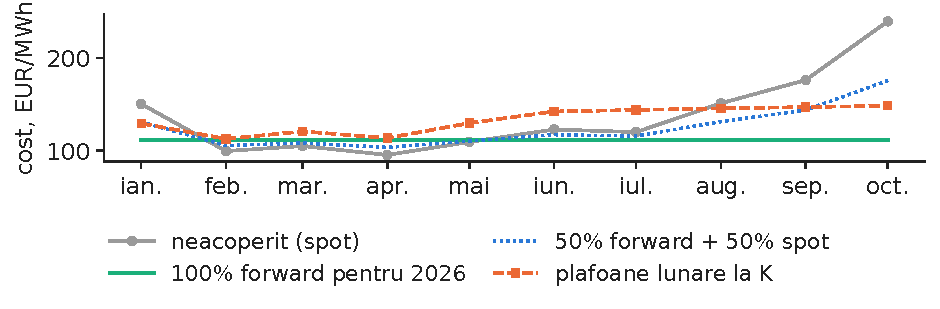
\includegraphics[width=\textwidth,height=0.561\textheight,keepaspectratio]{charts/ro/case2026.pdf}\end{center}\vspace{-3mm}
\chartsource{Sursa: OPCOM (rezultatele PCCB-LE-flex; prețuri PZU, prin energy-charts.info); BCE. Date: 2026-01 - 2026-10; 1 MW în bandă.}
\vspace{0.5mm}
\begin{itemize}\setlength{\itemsep}{0pt}
  \item Prețul spot a atins 239{,}3 EUR/MWh în octombrie 2026
    \begin{itemize}\setlength{\itemsep}{0pt}
      \item Plafoanele s-au exercitat în 5 din 10 luni.
    \end{itemize}
\end{itemize}
\par\vfill\manager{prima plafonului se plătește în fiecare lună, chiar și atunci cînd opțiunea nu se exercită.}\par\vspace{0.5mm}
\par\vfill\noindent{\scriptsize\color{FooterGray}(calcule proprii; OPCOM)}\hfill\qlink{EMQA\_L5\_case2026}{Quantlets/L5/EMQA_L5_case2026}\par\vspace{0.5mm}
\end{frame}

\begin{frame}{Studiul de caz: forward-ul a redus costul și riscul}
\footnotesize
\begin{columns}[T,onlytextwidth]
\begin{column}{0.50\textwidth}
{\footnotesize\renewcommand{\arraystretch}{1.25}\setlength{\tabcolsep}{4pt}
\begin{tabular}{@{}lrrrr@{}}\toprule
EUR/MWh & media & abat.\ std. & maxim & EUR/MW \\ \midrule
spot & 137{,}5 & 44{,}4 & 239{,}3 & 1\,002\,956 \\
100\% forward & 111{,}7 & 0{,}0 & 111{,}7 & 814\,946 \\
50\% forward & 124{,}6 & 22{,}2 & 175{,}5 & 908\,951 \\
plafoane & 133{,}6 & 13{,}9 & 148{,}5 & 975\,020 \\
\bottomrule\end{tabular}}
\par\vspace{0.5mm}{\scriptsize \begin{itemize}\setlength{\itemsep}{0pt}
  \item Ponderat cu numărul de ore al fiecărei luni.
\end{itemize}}
\end{column}
\begin{column}{0.47\textwidth}
\begin{itemize}\setlength{\itemsep}{1pt}
  \item \textbf{Interpretare}
    \begin{itemize}\setlength{\itemsep}{0pt}
      \item Forward: 188\,010 EUR economisiți pe MW, fără variație
      \item Plafoane: prima medie 20{,}4 EUR/MWh pe lună; economie netă 27\,936 EUR pe MW
    \end{itemize}
  \item \textbf{Nu este o regulă generală}
    \begin{itemize}\setlength{\itemsep}{0pt}
      \item Prețurile au crescut după acoperire; într-un an cu prețuri în scădere, forward-ul costă mai mult decît spotul
    \end{itemize}
\end{itemize}
\end{column}
\end{columns}
\par\vfill\manager{stabiliți ponderea acoperită prin politică (de exemplu 60--80\%, eșalonat), nu după o opinie despre prețuri.}\par\vspace{0.5mm}
\par\vfill\noindent{\scriptsize\color{FooterGray}(calcule proprii)}\hfill\tryit{notebook-ul Jupyter, secțiunea 7}\par\vspace{0.5mm}
\end{frame}

\begin{frame}{Perspectiva producătorului și saltul de preț din vara lui 2024}
\footnotesize
\begin{itemize}\setlength{\itemsep}{1pt}
  \item \textbf{Producătorul, 2025}
    \begin{itemize}\setlength{\itemsep}{0pt}
      \item 101 licitații, VWAP 102{,}1, față de media realizată de 108{,}2 EUR/MWh
      \item Vînzarea forward a adus cu 6{,}0 EUR/MWh mai puțin decît spotul (52\,797 EUR pe MW și an): prețul unui venit sigur
      \item În 2022, aceeași decizie a costat 187{,}9 EUR/MWh
    \end{itemize}
  \item \textbf{Vara lui 2024}
    \begin{itemize}\setlength{\itemsep}{0pt}
      \item Contractul pentru trimestrul al treilea s-a tranzacționat la 90{,}0 EUR/MWh, iar media spot realizată a fost 127{,}4; în iulie: 145{,}1
      \item Ora cea mai scumpă: 916{,}7 EUR/MWh, pe 18 iulie 2024, ora 20:00 ora Europei Centrale (CET)
    \end{itemize}
  \item \textbf{Concluzia}
    \begin{itemize}\setlength{\itemsep}{0pt}
      \item Acoperirea transferă valoare între cele două părți; face fluxurile de numerar previzibile, iar creditorii răsplătesc această previzibilitate prin condiții de finanțare mai bune
    \end{itemize}
\end{itemize}
\par\vfill\manager{un producător îndatorat ar trebui să vîndă forward chiar dacă se așteaptă la prețuri mai mari.}\par\vspace{0.5mm}
\par\vfill\noindent{\scriptsize\color{FooterGray}(calcule proprii; OPCOM; Andrei, Pele \& Cramer, 2026, PICBE)}\hfill\tryit{notebook-ul Jupyter, secțiunea 7}\par\vspace{0.5mm}
\end{frame}

\begin{frame}{Elementele unei politici de acoperire a riscului}
\footnotesize
\begin{columns}[T,onlytextwidth]
\begin{column}{0.50\textwidth}
\begin{itemize}\setlength{\itemsep}{1pt}
  \item \textbf{Expunerea}
    \begin{itemize}\setlength{\itemsep}{0pt}
      \item Poziția netă pe lună și pe profil (bandă, vîrf, solar)
      \item Riscul de volum: cererea reacționează foarte puțin la preț
    \end{itemize}
  \item \textbf{Instrumentele}
    \begin{itemize}\setlength{\itemsep}{0pt}
      \item Întîi forward OPCOM, apoi futures din Ungaria, apoi din Germania
      \item Plafoane pentru extreme, nu pentru tot volumul
    \end{itemize}
\end{itemize}
\end{column}
\begin{column}{0.47\textwidth}
\begin{itemize}\setlength{\itemsep}{1pt}
  \item \textbf{Execuția}
    \begin{itemize}\setlength{\itemsep}{0pt}
      \item Cumpărați eșalonat, pe 12--24 de luni
      \item Păstrați o rezervă de lichiditate pentru apelurile în marjă
    \end{itemize}
  \item \textbf{Controlul}
    \begin{itemize}\setlength{\itemsep}{0pt}
      \item Limite pentru poziția deschisă și VaR (cursul 4)
      \item Raportați costul acoperit și varianța lui
    \end{itemize}
\end{itemize}
\end{column}
\end{columns}
\par\vfill\manager{consiliul aprobă politica, traderii o execută, departamentul de risc o măsoară.}\par\vspace{0.5mm}
\par\vfill\noindent{\scriptsize\color{FooterGray}(Hull, 2022; Proșcanu, Proșcanu \& Pele, 2025, JSES; cursul 4)}\par\vspace{0.5mm}
\end{frame}

\section*{Recapitulare}

\begin{frame}{Test 1: riscul de bază}
\small
\begin{itemize}
  \item Un furnizor din România și-a acoperit luna iulie 2024 cu contracte futures germane în bandă, cumpărate la prețul $F$
    \begin{itemize}\setlength{\itemsep}{0pt}
      \item Media lunii a fost 67{,}7 în Germania și 145{,}1 EUR/MWh în România
      \item Cît a plătit pe MWh?
    \end{itemize}
\end{itemize}
\vspace{2mm}
\begin{exampleblock}{R\u{a}spuns}
\begin{itemize}
  \item A cumpărat la 145{,}1 în România și a primit din contractul futures diferența dintre 67{,}7 și $F$: costul net este $F$ + 77{,}4 EUR/MWh, cea mai mare bază lunară din datele noastre.
\end{itemize}
\end{exampleblock}
\end{frame}

\begin{frame}{Test 2: raportul de acoperire}
\small
\begin{itemize}
  \item Estimarea noastră pentru Ungaria este $h^{*}$ = 0{,}966, cu intervalul bootstrap [0{,}93; 1{,}03]
    \begin{itemize}\setlength{\itemsep}{0pt}
      \item Cîți MW de contracte futures din Ungaria acoperă o expunere de 20 MW?
    \end{itemize}
\end{itemize}
\vspace{2mm}
\begin{exampleblock}{R\u{a}spuns}
\begin{itemize}
  \item 20 $\times$ 0{,}966 = 19{,}3 MW
    \begin{itemize}\setlength{\itemsep}{0pt}
      \item Deoarece valoarea 1 se află în interval, o acoperire integrală ($h=1$), de 20 MW, este la fel de bună din punct de vedere statistic.
    \end{itemize}
\end{itemize}
\end{exampleblock}
\end{frame}

\begin{frame}{Test 3: clean spark spread}
\small
\begin{itemize}
  \item În octombrie 2026: energia 239{,}3, gazele 86{,}8 EUR/MWh, EUA 82{,}4 EUR/t
    \begin{itemize}\setlength{\itemsep}{0pt}
      \item Randament 50\%, 0,202 t CO$_2$ pe MWh termic
      \item A cîștigat, în medie, o centrală pe gaze?
    \end{itemize}
\end{itemize}
\vspace{2mm}
\begin{exampleblock}{R\u{a}spuns}
\begin{itemize}
  \item Combustibilul: 86{,}8/0,5 = 173{,}6
    \begin{itemize}\setlength{\itemsep}{0pt}
      \item Carbonul: 0,404 $\times$ 82{,}4 = 33{,}3
      \item Clean spark spread \ensuremath{+}32{,}4 EUR/MWh: da, chiar înainte de a alege orele cele mai bune.
    \end{itemize}
\end{itemize}
\end{exampleblock}
\end{frame}

\begin{frame}{Test 4: un plafon pentru un furnizor}
\small
\begin{itemize}
  \item Banda pentru 2027 se tranzacționează la 148{,}1
    \begin{itemize}\setlength{\itemsep}{0pt}
      \item Un plafon la 162{,}9 costă 0{,}63 EUR/MWh
      \item Cît plătește furnizorul dacă prețul forward ajunge la 1,3 $F$, respectiv la 0,9 $F$?
    \end{itemize}
\end{itemize}
\vspace{2mm}
\begin{exampleblock}{R\u{a}spuns}
\begin{itemize}
  \item La 1,3 $F$: prețul de exercitare de 162{,}9 plus prima
    \begin{itemize}\setlength{\itemsep}{0pt}
      \item La 0,9 $F$: prețul pieței plus prima, deoarece plafonul nu se exercită.
    \end{itemize}
\end{itemize}
\end{exampleblock}
\end{frame}

\begin{frame}{Recapitulare}
\small
\vspace{-2mm}\begin{multicols}{2}\scriptsize\tableofcontents\end{multicols}
\begin{itemize}\setlength{\itemsep}{1pt}
  \item Un contract forward transformă un preț spot necunoscut într-un preț cunoscut
    \begin{itemize}\setlength{\itemsep}{0pt}
      \item În 2022 i-a adus unui furnizor din România o economie de 1{,}65 milioane EUR pe MW, iar producătorii care au vîndut forward au pierdut aceeași sumă.
    \end{itemize}
  \item Acoperiți riscul din România cu contracte din Ungaria, înaintea celor din Germania
    \begin{itemize}\setlength{\itemsep}{0pt}
      \item Includeți profilul în preț și alegeți volatilitatea potrivită activului suport
      \item Urmează cursul 6.
    \end{itemize}
\end{itemize}
\end{frame}

\begin{frame}{Cercetările grupului nostru despre riscul pe piața energiei din România}
\footnotesize
\begin{itemize}\setlength{\itemsep}{1pt}
  \item \textbf{Saltul de preț din vara lui 2024} (Andrei, Pele \& Cramer, 2026, PICBE)
    \begin{itemize}\setlength{\itemsep}{0pt}
      \item Întrebarea: ce intervenție ar fi redus cel mai mult prețurile din România în iunie--iulie 2024
      \item Metoda: o pădure aleatoare (random forest) pe date orare ENTSO-E, 147 de scenarii contrafactuale, verificate cu o regresie ridge
      \item Rezultatul: reducerea consumului cu 10\% este cea mai eficientă măsură; vîrful a avut loc noaptea, deci energia solară nu putea ajuta, iar stocarea devine esențială
    \end{itemize}
  \item \textbf{Riscul sistemic în sectorul energetic din UE} (Toma, Dima, Grecu, Pele \& Lessmann, 2026, SSRN)
    \begin{itemize}\setlength{\itemsep}{0pt}
      \item Metoda: indicatorul Energy Financial Risk Meter, construit prin regresie cuantilică cu operatorul de contracție și selecție în normă absolută (LASSO) pe randamentele zilnice a 100 de companii energetice europene
      \item Rezultatul: indicele surprinde pandemia din 2020 și războiul din 2022; se activează un canal de transmitere a riscului geopolitic către sectorul energetic
    \end{itemize}
  \item \textbf{Cererea reacționează foarte puțin la preț} (Proșcanu, Proșcanu \& Pele, 2025, JSES)
    \begin{itemize}\setlength{\itemsep}{0pt}
      \item Metoda: cauzalitate Granger și modele vectoriale autoregresive pe consumul și prețurile din România
      \item Rezultatul: consumul este inelastic și influențează prețul, nu invers; de aceea volumul nu poate compensa riscul de preț
    \end{itemize}
\end{itemize}
\par\vspace{0.5mm}{\scriptsize \begin{itemize}\setlength{\itemsep}{0pt}
  \item Rezultatele de pe acest diapozitiv sînt cele raportate în lucrări; celelalte cifre din curs provin din calculele noastre.
\end{itemize}}
\par\vfill\noindent{\scriptsize\color{FooterGray}(Academia de Studii Economice din București; Academia Română, Institutul de Prognoză Economică)}\par\vspace{0.5mm}
\end{frame}

\begin{frame}{Lecturi și resurse suplimentare}
\small
\begin{columns}[T,onlytextwidth]
\begin{column}{0.52\textwidth}
\begin{itemize}\setlength{\itemsep}{1pt}
  \item \textbf{J.\ Hull, Options, Futures, and Other Derivatives}, capitolele despre acoperirea riscului, contracte futures și modelul Black.
  \item \textbf{Benth, Šaltytė Benth \& Koekebakker (2008)}: curbe forward și opțiuni pe piețele de energie electrică.
  \item \textbf{Rapoartele OPCOM}: rezultatele licitațiilor forward, sursa acestui curs --- \href{https://www.opcom.ro/rapoarte-pccb-le-flex-rez-pccb-le-flex/ro}{opcom.ro}.
\end{itemize}
\end{column}
\begin{column}{0.45\textwidth}
\begin{itemize}\setlength{\itemsep}{1pt}
  \item \textbf{Acest curs}: cod, date, notebook-uri Jupyter --- \href{https://github.com/danpele/EMQA}{github.com/danpele/EMQA}.
  \item \textbf{ACER (2022)}: evaluarea finală a modelului pieței angro de energie electrică din UE.
  \item \textbf{Exercițiu practic}: notebook-ul Jupyter reproduce toate graficele și cifrele din acest curs --- \href{\emqarepo/\emqanb}{notebooks/}.
\end{itemize}
\end{column}
\end{columns}
\end{frame}

\begin{frame}{Bibliografie (1/3)}
\scriptsize
\begin{itemize}\setlength{\itemsep}{1pt}\scriptsize
\item ACER (2022). \textit{ACER's Final Assessment of the EU Wholesale Electricity Market Design}. Ljubljana, April 2022. \href{https://www.acer.europa.eu/events-and-engagement/news/press-release-acer-publishes-its-final-assessment-eu-wholesale}{acer.europa.eu}
\item Andrei, A.-V., Pele, D.-T.\ \& Cramer, A.-A.\ (2026). Evaluating intervention effectiveness during extreme price events: A counterfactual analysis of Romania's 2024 energy crisis. \textit{Proceedings of the International Conference on Business Excellence}, 20(1), 84--103. \href{https://doi.org/10.2478/picbe-2026-0013}{doi:10.2478/picbe-2026-0013}
\item Benth, F.\,E., Šaltytė Benth, J.\ \& Koekebakker, S.\ (2008). \textit{Stochastic Modeling of Electricity and Related Markets}. World Scientific. \href{https://doi.org/10.1142/6811}{doi:10.1142/6811}
\item Bessembinder, H.\ \& Lemmon, M.\,L.\ (2002). Equilibrium pricing and optimal hedging in electricity forward markets. \textit{Journal of Finance}, 57(3), 1347--1382. \href{https://doi.org/10.1111/1540-6261.00463}{doi:10.1111/1540-6261.00463}
\item Black, F.\ (1976). The pricing of commodity contracts. \textit{Journal of Financial Economics}, 3(1--2), 167--179. \href{https://doi.org/10.1016/0304-405X(76)90024-6}{doi:10.1016/0304-405X(76)90024-6}
\item Deng, S.-J., Johnson, B.\ \& Sogomonian, A.\ (2001). Exotic electricity options and the valuation of electricity generation and transmission assets. \textit{Decision Support Systems}, 30(3), 383--392. \href{https://doi.org/10.1016/S0167-9236(00)00112-3}{doi:10.1016/S0167-9236(00)00112-3}
\item Ederington, L.\,H.\ (1979). The hedging performance of the new futures markets. \textit{Journal of Finance}, 34(1), 157--170. \href{https://doi.org/10.1111/j.1540-6261.1979.tb02077.x}{doi:10.1111/j.1540-6261.1979.tb02077.x}
\item ENTSO-E (2021). Successful go-live of Interim Coupling, reaching the SDAC enduring phase. Press release, 18 June 2021. \href{https://www.entsoe.eu/news/2021/06/18/successful-go-live-of-interim-coupling-reaching-the-sdac-enduring-phase/}{entsoe.eu}
\end{itemize}
\end{frame}

\begin{frame}{Bibliografie (2/3)}
\scriptsize
\begin{itemize}\setlength{\itemsep}{1pt}\scriptsize
\item Eydeland, A.\ \& Wolyniec, K.\ (2003). \textit{Energy and Power Risk Management: New Developments in Modeling, Pricing, and Hedging}. Wiley. \href{https://www.wiley.com/en-us/Energy+and+Power+Risk+Management-p-9780471104001}{wiley.com}
\item Fama, E.\,F.\ \& French, K.\,R.\ (1987). Commodity futures prices: Some evidence on forecast power, premiums, and the theory of storage. \textit{Journal of Business}, 60(1), 55--73. \href{https://doi.org/10.1086/296385}{doi:10.1086/296385}
\item Hull, J.\,C.\ (2022). \textit{Options, Futures, and Other Derivatives}, 11th ed. Pearson. \href{https://www.pearson.com/en-us/subject-catalog/p/options-futures-and-other-derivatives/P200000005938}{pearson.com}
\item IPCC (2006). \textit{2006 IPCC Guidelines for National Greenhouse Gas Inventories}, Vol.\ 2 Energy, ch.\ 2, Table 2.2 (default emission factors). \href{https://www.ipcc-nggip.iges.or.jp/public/2006gl/pdf/2_Volume2/V2_2_Ch2_Stationary_Combustion.pdf}{ipcc-nggip.iges.or.jp}
\item Johnson, L.\,L.\ (1960). The theory of hedging and speculation in commodity futures. \textit{Review of Economic Studies}, 27(3), 139--151. \href{https://doi.org/10.2307/2296076}{doi:10.2307/2296076}
\item Kroner, K.\,F.\ \& Sultan, J.\ (1993). Time-varying distributions and dynamic hedging with foreign currency futures. \textit{Journal of Financial and Quantitative Analysis}, 28(4), 535--551. \href{https://doi.org/10.2307/2331164}{doi:10.2307/2331164}
\item Longstaff, F.\,A.\ \& Wang, A.\,W.\ (2004). Electricity forward prices: A high-frequency empirical analysis. \textit{Journal of Finance}, 59(4), 1877--1900. \href{https://doi.org/10.1111/j.1540-6261.2004.00682.x}{doi:10.1111/j.1540-6261.2004.00682.x}
\item Margrabe, W.\ (1978). The value of an option to exchange one asset for another. \textit{Journal of Finance}, 33(1), 177--186. \href{https://doi.org/10.1111/j.1540-6261.1978.tb03397.x}{doi:10.1111/j.1540-6261.1978.tb03397.x}
\end{itemize}
\end{frame}

\begin{frame}{Bibliografie (3/3)}
\scriptsize
\begin{itemize}\setlength{\itemsep}{1pt}\scriptsize
\item OUG 27/2022 privind măsurile aplicabile clienților finali din piața de energie electrică și gaze naturale (Monitorul Oficial nr.\ 274, 22 martie 2022); OUG 153/2022 (MACEE). \href{https://legislatie.just.ro}{legislatie.just.ro}
\item Proșcanu, C., Proșcanu, M.\ \& Pele, D.\,T.\ (2025). The price elasticity of electricity demand in Romania. \textit{Journal of Social and Economic Statistics}, 14(2), 131--141. \href{https://doi.org/10.2478/jses-2025-0009}{doi:10.2478/jses-2025-0009}
\item Redl, C., Haas, R., Huber, C.\ \& Böhm, B.\ (2009). Price formation in electricity forward markets and the relevance of systematic forecast errors. \textit{Energy Economics}, 31(3), 356--364. \href{https://doi.org/10.1016/j.eneco.2008.12.001}{doi:10.1016/j.eneco.2008.12.001}
\item Samuelson, P.\,A.\ (1965). Proof that properly anticipated prices fluctuate randomly. \textit{Industrial Management Review}, 6(2), 41--49; reprinted in \textit{World Scientific Handbook in Financial Economics} (2015), 25--38. \href{https://doi.org/10.1142/9789814566926_0002}{doi:10.1142/9789814566926\_0002}
\item Schwartz, E.\,S.\ (1997). The stochastic behavior of commodity prices: Implications for valuation and hedging. \textit{Journal of Finance}, 52(3), 923--973. \href{https://doi.org/10.1111/j.1540-6261.1997.tb02721.x}{doi:10.1111/j.1540-6261.1997.tb02721.x}
\item Toma, F.-M., Dima, D.\,M., Grecu, R., Pele, D.\,T.\ \& Lessmann, S.\ (2026). Energy Financial Risk Meter: Systemic risk in the EU energy sector. SSRN working paper. \href{https://doi.org/10.2139/ssrn.6985301}{doi:10.2139/ssrn.6985301}
\item Weron, R.\ (2008). Market price of risk implied by Asian-style electricity options and futures. \textit{Energy Economics}, 30(3), 1098--1115. \href{https://doi.org/10.1016/j.eneco.2007.05.004}{doi:10.1016/j.eneco.2007.05.004}
\end{itemize}
\end{frame}

\appendix

\section*{Anexă}

\begin{frame}{Anexa A: raportul de acoperire cu varianță minimă și estimarea lui}
\small
\begin{columns}[T,onlytextwidth]
\begin{column}{0.54\textwidth}
\[ \frac{\partial}{\partial h}\Var(\Delta S-h\Delta F)=-2\Cov(\Delta S,\Delta F)+2h\Var(\Delta F)=0 \]\[ \Rightarrow\ h^{*}=\frac{\Cov(\Delta S,\Delta F)}{\Var(\Delta F)} \]\[ \Var(\Delta S-h^{*}\Delta F)=\sigma_S^2(1-\rho^2) \]\begin{itemize}\setlength{\itemsep}{1pt}
  \item A doua derivată, $2\Var(\Delta F)>0$, deci $h^{*}$ este un minim.
  \item $h^{*}$ este panta OLS a regresiei lui $\Delta S$ pe $\Delta F$
    \begin{itemize}\setlength{\itemsep}{0pt}
      \item Varianța HAC (Newey--West, nucleu Bartlett, 3 decalaje).
    \end{itemize}
\end{itemize}
\end{column}
\begin{column}{0.43\textwidth}
\begin{itemize}\setlength{\itemsep}{1pt}
  \item \textbf{Bootstrap pe blocuri mobile}
    \begin{itemize}\setlength{\itemsep}{0pt}
      \item Se extrag cu întoarcere blocuri de cîte 6 luni consecutive pînă la $n$ luni; se recalculează $h^{*}$; procedura se repetă de 2\,000 de ori
      \item Intervalul de 95\% = percentilele de 2,5\% și 97,5\%; blocurile păstrează autocorelarea variațiilor lunare
    \end{itemize}
  \item \textbf{Rapoarte de acoperire dinamice}
    \begin{itemize}\setlength{\itemsep}{0pt}
      \item $h_t^{*}=\Cov_{t-1}/\Var_{t-1}$, dintr-un model GARCH bivariat (cursul 3)
    \end{itemize}
\end{itemize}
\end{column}
\end{columns}
\par\vfill\noindent{\scriptsize\color{FooterGray}(Johnson, 1960; Ederington, 1979; Kroner \& Sultan, 1993)}\par\vspace{0.5mm}
\end{frame}

\begin{frame}{Anexa B: de la un preț forward fără tendință la formula Black-76}
\small
\begin{columns}[T,onlytextwidth]
\begin{column}{0.54\textwidth}
\[ \frac{dF_t}{F_t}=\sigma\,dW_t\ \Rightarrow\ \ln F_T\sim\mathcal N\big(\ln F_0-\tfrac12\sigma^2T,\ \sigma^2T\big) \]\[ C=e^{-rT}\E\big[(F_T-K)^+\big]=e^{-rT}\big[F_0\Phi(d_1)-K\Phi(d_2)\big] \]\begin{itemize}\setlength{\itemsep}{1pt}
  \item Intrarea într-un contract forward nu costă nimic, deci în evaluarea neutră la risc tendința lui este zero.
  \item $\E[F_T\mathbf 1_{F_T>K}]=F_0\Phi(d_1)$ și $\Pr(F_T>K)=\Phi(d_2)$ (momentele repartiției lognormale).
\end{itemize}
\end{column}
\begin{column}{0.43\textwidth}
\begin{itemize}\setlength{\itemsep}{1pt}
  \item \textbf{Opțiuni pe marjă}
    \begin{itemize}\setlength{\itemsep}{0pt}
      \item Opțiunea de a schimba gazele în energie: formula Margrabe, cu $\sigma^2=\sigma_P^2+\sigma_G^2-2\rho\sigma_P\sigma_G$
      \item Dacă există și un preț de exercitare (de exemplu, costurile variabile ale centralei), în practică se folosește aproximarea Kirk
    \end{itemize}
  \item \textbf{Revenirea la medie}
    \begin{itemize}\setlength{\itemsep}{0pt}
      \item Prețul spot revine la medie; modelul cu un factor al lui Schwartz (1997) dă volatilități forward care scad cu scadența
    \end{itemize}
\end{itemize}
\end{column}
\end{columns}
\par\vfill\noindent{\scriptsize\color{FooterGray}(Black, 1976; Margrabe, 1978; Schwartz, 1997)}\par\vspace{0.5mm}
\end{frame}

\begin{frame}{Anexa C: convenții și factori de conversie}
\footnotesize
\begin{itemize}\setlength{\itemsep}{1pt}
  \item \textbf{Prețurile forward}
    \begin{itemize}\setlength{\itemsep}{0pt}
      \item Un preț de închidere pentru fiecare sesiune OPCOM; volumul tranzacționat, înregistrat pe partea inițiatorului licitației; conversia din lei cu cursul BCE din ziua licitației (ultimul curs disponibil)
      \item Numai perioade standard: lună, trimestru, semestru, an calendaristic; în bandă, dacă nu se precizează altfel
    \end{itemize}
  \item \textbf{Spotul realizat}
    \begin{itemize}\setlength{\itemsep}{0pt}
      \item Media prețurilor zilnice în bandă de pe PZU din perioada de livrare (zile CET); se calculează numai dacă toate zilele sînt disponibile
    \end{itemize}
  \item \textbf{Combustibili și carbon}
    \begin{itemize}\setlength{\itemsep}{0pt}
      \item Cărbune de 6\,000 kcal/kg = 6,978 MWh termic pe tonă; gaze 0,202 și cărbune 0,341 t CO$_2$ pe MWh termic (IPCC 2006: 56,1 și 94,6 t/TJ)
      \item EUA = media lunară a licitațiilor EEX pînă în ianuarie 2026, apoi titlul SparkChange ETC (raportul licitație/ETC este apropiat de 1 în 2021--2025)
    \end{itemize}
  \item \textbf{Ore}
    \begin{itemize}\setlength{\itemsep}{0pt}
      \item Echivalent orar: un interval de 15 minute contează ca 0,25 h (din 1 octombrie 2025)
    \end{itemize}
\end{itemize}
\par\vfill\noindent{\scriptsize\color{FooterGray}(IPCC, 2006; OPCOM; BCE)}\par\vspace{0.5mm}
\end{frame}

\end{document}
